\documentclass[11pt,letterpaper]{article}

\usepackage{tabularx,booktabs}
\usepackage{url}
\usepackage{fullpage}
\usepackage{graphicx}
\usepackage{lipsum}
\usepackage{booktabs} % For formal tables
\usepackage{algorithm}
\usepackage{algorithmic}
\usepackage{amsmath}
\usepackage{multirow, makecell}
\usepackage{url}
\usepackage{flushend}
\usepackage{comment}
\usepackage{xspace}
\usepackage{adjustbox}
\usepackage{color}
%\usepackage{caption2}
\usepackage{enumitem}
\usepackage{caption}
\captionsetup{font=footnotesize}
\usepackage[margin=1in]{geometry}

\newcommand{\junk}[1]{}

\newcommand{\name}{{\sc Athena}\xspace}

\newcommand{\ie}{\emph{i.e.}\xspace}
\newcommand{\eg}{\emph{e.g.}\xspace}
\newcommand{\SCcomment}[1]{{\textcolor{red}{\bf [SC: #1]}}}
\newcommand{\AMcomment}[1]{{\textcolor{blue}{\bf [AM: #1]}}}

\begin{document}
\thispagestyle{empty}

\title{\textit{\name}: Automated Tuning of Genomic Error Correction Algorithms using Language Models}


\author
{
\centering
Mustafa Abdallah$^{*1}$  \and Ashraf Mahgoub$^{*2}$ 
\and Saurabh Bagchi$^{1}$ \and Somali Chaterji$^{1}$ 
\\
		$^{1}$School of Electrical and Computer Engineering\\
	   	$^{2}$Department of Computer Science\\
                Purdue University\\
{\small $^*$ The first two authors contributed equally to the work.}
}

\date{}

\maketitle
\begin{abstract}
  \noindent {The performance of most error-correction algorithms that operate on genomic sequencer reads is dependent on the proper choice of its configuration parameters, such as the value of $k$ in \textit{k}-mer based techniques.} In this work, we target the problem of finding the best values of these configuration parameters to optimize error correction.
We perform this in a data-driven manner, due to the observation that different configuration parameters are optimal for different datasets, \ie different instruments and organisms. 
%, and more importantly, downstream genome assembly. %have not used genome assembly now so misleading/removed (SC10302018)
We use language modeling techniques from the Natural Language Processing (NLP) domain in our algorithmic suite, \textsc{Athena}, to automatically tune the performance-sensitive configuration parameters. Through the use of N-Gram and Recurrent Neural Network (RNN) language modeling, we validate the intuition that the quality of the correction can be computed quantitatively and efficiently using the ``perplexity'' metric, prevalent in the NLP domain. After training the language model, we show that the perplexity metric calculated for runtime data has a strong negative correlation with the correction of the erroneous NGS reads. Therefore, we use the perplexity metric to guide a hill climbing-based search, converging toward the best $k$-value. Our approach is suitable for both \textit{de novo} and comparative sequencing (resequencing), eliminating the need for a reference genome to serve as the ground truth. This is important because use of a reference genome often carries forward the biases along the stages of the pipeline. Further, in more specialized applications such as variant-calling, a reference genome may in fact be misleading, making \name suitable for such applications. %\SCcomment{So, this last line shows why our method is useful even in comparative seq and some other applications}
% Mus: Makes sense.

\end{abstract}

\section{Introduction}
\begin{figure}
\centering
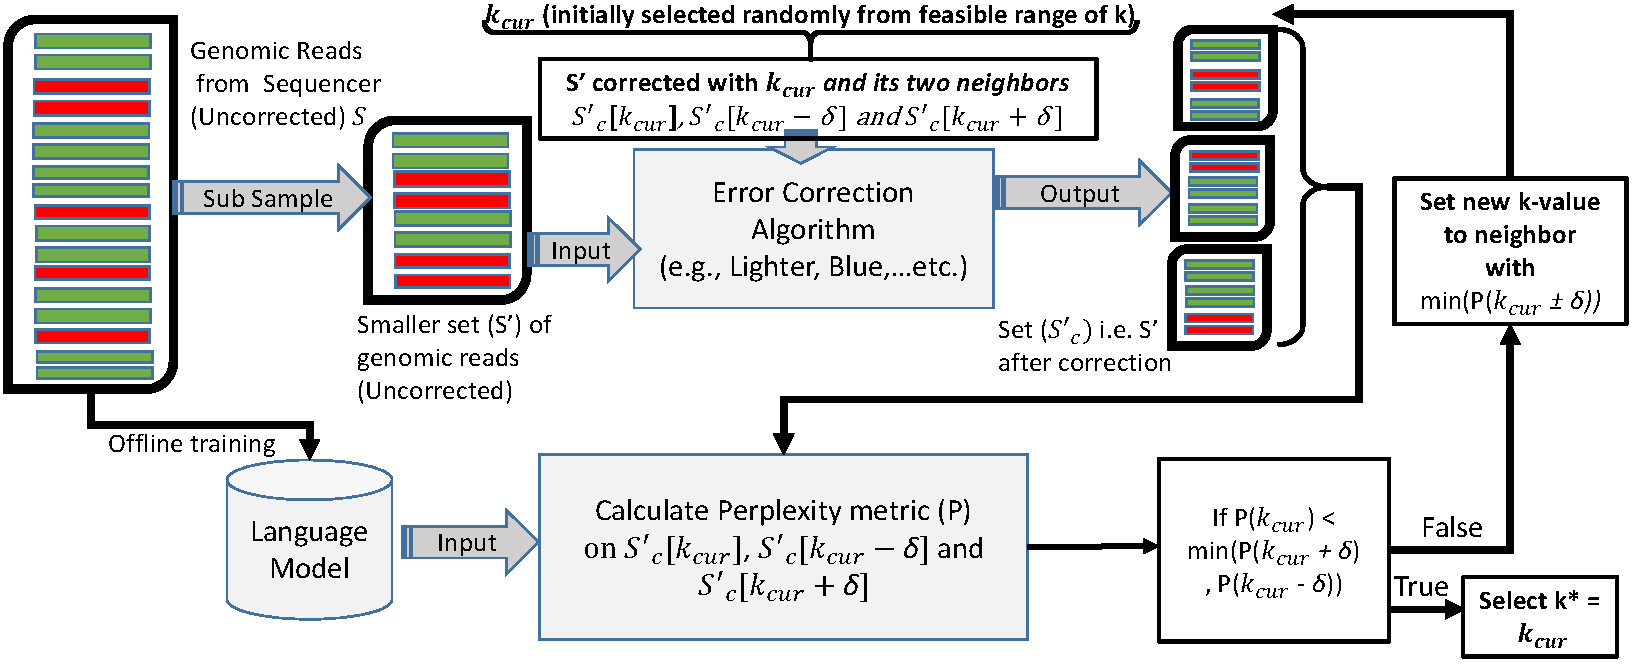
\includegraphics[width=\linewidth]{figs/AthenaOverview_Compressed2_cropped.pdf}
\caption{Overview of \name's workflow. First, we train the language model using the entire set of uncorrected reads for the specific dataset. Second, we perform error correction on a sub-sample from the uncorrected reads using an EC tool (\eg Lighter or Blue) and a range of $k$-values. Third, we evaluate the perplexity of each corrected sample and decide on the best $k$-value for the next iteration, \ie the one corresponding to the lowest perplexity metric because error correction quality is negatively correlated with the perplexity metric. This process continues until the termination criteria are met. Finally, the complete set of reads is corrected with the best $k$-value found.}	
\label{fig:AthenaOverview}
\end{figure}
\vspace{-10pt}
Rapid advances in genome sequencing technologies, with the resulting drops in sequencing costs, offer unprecedented opportunities to characterize genomes across the tree of life. %The first sequencing of the human whole genome (in 2003) cost roughly \$2.7 billion, reducing to the current thousand dollar regime, and further aspirations by Illumina to sequence the whole genome for less than \$100. This sharp drop in sequencing and operational costs is being fueled by the surge in powerful computing machines and optimized laboratory and computational processing techniques in recent years. 
While next-generation sequencing (NGS) techniques allow for rapid parallel sequencing vis-$\grave{a}$-vis older methods, NGS reads are more error-prone, especially for more complex genomes. %with exact or almost-exact repeat regions. 
In addition, sequencing platforms generate reads with different error profiles, including incorrect base replacements, insertions, deletions, etc. The current bottleneck of NGS projects is not the DNA sequencing process itself but the structured data management and sophisticated computational analysis downstream \cite{schadt2010computational}. In order to get biologically meaningful results, each step of the analysis workflow needs to be analyzed so errors are not magnified along the analysis pipeline.
% differing in size or copy number.
% SB (1/27/18): It may be better to talk of ``next generation sequencing'' than ``shotgun sequencing'' since our solution is even more applicable there. 
Consequently, multiple error-correction (EC) techniques have been developed to correct NGS reads in order to improve downstream applications, including genome assembly and variant calling \cite{szalay2015novo}. 

Genomic read correction is computationally expensive, especially for short-read sequencing ($\leq$ 100-bp long), requiring high sequencing coverage, and with common applications in metagenomics and meta-transcriptomics \cite{meyer2017mg,chaterji2017federation}.
% SB (11/3/18): Why is EC expensive for short-read sequencing? I think the relevant factor is how many base pairs are in the read set. So if we have short-read sequencing and high coverage, that leads to large number of base pairs and hence short-read sequencing in expensive then. But it does not have to do with short-read sequency per se.
% SB (11/3/18): I do not understand the relevance of the part ``and with common applications ...''.
The performance of many EC algorithms is highly dependent on the proper choice of configuration parameters, such as the value of $k$ (length of the substring) in \textit{k}-spectrum-based techniques \cite{mahadik2017scalable}, where the original genomic reads are split into overlapping sub-strings of size $k$. By extracting these $k$-mers from sequenced reads, an efficient \textit{de Bruijn} Graph (DBG) \cite{compeau2011apply} can be built for genome assembly. Selecting different values of $k$ has a trade-off. Having small values of $k$ increases the overlap probability between reads. However, an unsuitably small value of $k$ degrades the EC performance because it does not allow the algorithm to discriminate between correct and erroneous $k$-mers. On the other hand, having unsuitably high $k$-values decreases the overlap probability and hurts EC performance \cite{sameith2016iterative}. This is because most $k$-mers will appear unique and thus not allow us to distinguish legitimate and erroneous $k$-mers. 
The $k$-mers that appear above a certain threshold frequency, and are therefore expected to be legitimate, are called \textit{solid k-mers}. The others are called \textit{insolid or untrusted $k$-mers}. (In $k$-spectrum-based methods, the goal is to convert insolid $k$-mers to solid ones with a minimum number of edit operations.) Both increasing or decreasing the overlap probability affects the EC capability and hence, there is an optimum value of $k$ to use. Further, this value changes with the dataset or the organism whose genome is being sequenced \cite{heydari2017evaluation}. Moreover, most EC tools are evaluated based on their direct ability on reducing error rates rather than improving the genome assembly \cite{heydari2017evaluation}. Although the assembly can benefit substantially from EC tools, miscorrected reads can often result in degraded assemblies from formation of incorrect chimera etc. \cite{heydari2017evaluation}.
% SB (11/3/18): The above sentence should be made more general - good EC can benefit all these applications - assembly and name others too. ``Formation of incorrect chimera'' is too specific and can be dropped. 
%\SCcomment{can sub-optimal values of k result in miscorrected errors? if so, show the plot you have a miscorrected read resulting in worse assembly than the uncorrected read.}
%\AMcomment{Added a citation}
% Consequently, 
%In our paper, we show that \name can automatically find the best values of k-mer sizes for a given dataset which improves the quality of the generated assemblies. % For example, authors in KmerGenie \CITE{chikhi2013informed} found that $k=61$ for the human chromosome 14 ``chr14'' data set improves the quality of assembly by 35\% over using $k=51$. On the contrary, using $k=61$ with the  \textit{Bombus impatiens} ``\textit{B. impatiens}'' data set {\em reduces} the quality of assembly by 8.6\% over using $k=51$. Thus, the optimum $k$ value selection must be done for each data set.
%Another important factor is that the performance often degrades sharply with divergence of the $k$ value away from the optimal value. Thus, the optimal value of $k$ for the Velvet assembler with the ``chr14'' data set, when applied to the same assembler with the ``S.  aureus'' data set gives an assembly quality that is degraded by 75\%. 
%\SCcomment{data-driven method instead of saying automated?}
% Mus: Done.
Therefore, a data-driven  method for finding the best value of \textit{k} and other configuration parameters is needed for improved error correction, and subsequently, for superior genome alignment, genome assembly, variant calling, and other applications downstream.
% SB (11/3/18): Added alignment which we do evaluate. 
% \SCcomment{we don't evaluate genome assembly, so a little dicey to say this}.
%\AMcomment{Moreover, several EC tools depend on not a single, but a set of configuration parameters that control the quality of the correction process. For example, Reptile has five performance-sensitive parameters and our technique can optimize the values of multiple configuration parameters, with their dependencies.(CFC as we don't show any exp. with many configs}
%\SCcomment{\name can model dependencies, right?}\AMcomment{I don't think so}
% (e.g., gain). 
%SC(05/19/08): little bit of a stretch in that last part but it does not make sense to have those 2 sentences in there otherwise, making the claim above makes our technique shine though, so good to have.

%better word choice? I put automated (SC) 

% \begin{figure}
%   \includegraphics[width=\linewidth]{Figures/Kmer_Genie.eps}
%   \caption{Adapted from \cite{chikhi2013informed}: Best value of $k$ found by Kmer-genie for genome assembly for three data sets: \textit{S. aureus} (Velvet), chr14 (Velvet), and \textit{B.impatiens} (SOAPdenovo2)}
%   \label{fig:Best_K_Different_Data_Sets}
% \end{figure}

% SB (1/27/18): Why?  Give concrete proof that a good k value for one dataset (one organism?) can give a bad assembly for another dataset. This can be done by showing assembly quality is bad for one and good for another.  


% Sensitivity is a less stringent measure as it is equivalent to number of reads containing errors and  was classified as True Positive irrespective of whether they were accurately corrected or not.

% SB (1/27/18): Define sensitivity and gain in the figure caption. 

% \begin{figure*}%[!tpb]%figure1
% %\fboxsep=0pt\colorbox{gray}{\begin{minipage}[t]{235pt} \vbox to 100pt{\vfill\hbox to
% %235pt{\hfill\fontsize{24pt}{24pt}\selectfont FPO\hfill}\vfill}
% %\end{minipage}}
% \centerline{\includegraphicss[width=0.8\textwidth]{Figures/Athena_Overview.pdf}}
% \caption{Overview of Athena Workflow}
% \end{figure*}


Many existing EC solutions (\textit{e.g.}, Reptile \cite{yang2010reptile}, Quake \cite{kelley2010quake}, Lighter \cite{song2014lighter}, Blue \cite{greenfield2014blue}) require users to specify $k$. The best value is usually found by exploration over a range of $k$ values \cite{kao2011echo} and evaluating the performance metric--- \eg EC Gain, Alignment Rate, Accuracy, Recall, and Precision \cite{heydari2017evaluation}.
% The domain-specific parameter ``gain'' measures the percentage of errors effectively removed from the data set.
However, a reference genome is typically needed to serve as ground truth for evaluation, which makes this approach infeasible for \textit{de novo} sequencing tasks or where a high-quality reference genome is unavailable. 
%SC(05/21/18): do novo used likelihood-based metrics, so not accurately written above
% SB (5/21/18): But de novo does not need reference genome. Likelihood based metrics are calculated without taking recourse to a reference genome. 
To the best of our knowledge, existing tools leave the best parameter choice to the end user~\cite{peng2010idba, mahadik2017scalable}; a small number provide intuitive histograms or heuristics to assist in the decision process~\cite{chikhi2013informed}.
% SB (11/3/18): Add one or two more citations that provide such help. 
Thus, the need for a data-driven method to select the optimal $k$-value is crucial.
\SBcomment{Provide a motivating quantitative result - one value of k good for one dataset gives really bad result with another dataset.}

Our solution, {\em \name}\footnote{Just as \textit{Athena} is the Greek Goddess of wisdom and a fierce warrior, we wish our technique to unearth the genomic codes underlying disease in a fearless war against maladies.} finds the best value of the configuration parameters
for correcting errors in genome sequencing, such as the value of $k$ in $k$-mer based methods. Further, \name does not require access to a reference genome to perform its function of determining the optimal parameter configuration\footnote{In our evaluation, we use Bowtie2 to perform alignment and then measure the alignment rate as the metric to evaluate our solution. But alignment is not needed for \name to work.}. 
% genome to compute the quality of the corrected reads, although we use Bowtie to align against the reference genome for evaluation.
This makes it much faster compared to existing \textit{de novo} assembly quality metrics such as CGAL \cite{rahman2013cgal} and ALE \cite{clark2013ale}.
% SB (11/3/18): I do not understand the above sentence. This seems like an apples-to-oranges comparison - we are doing error correction and you are comparing it to assembly. Also, what does it mean to be faster than a metric?
%Thus, \name improves the performance of the error correction phase, which also improves the quality of genome assembly approaches---\textit{de novo} and comparative (reference-based) genome assembly. %\AMcomment{Why making it faster improves the performance and quality of assembly?} SC-- no it does not.. I don't recall writing this.
%During comparative genome assembly, a reference genome from the same or a closely related species is used to map the assembly process by aligning the fragments being assembled. Using \name for comparative sequencing obviates the need to use this reference genome. 
In the case of \textit{de novo} assembly, \name takes advantage of the fact that NGS reads have the property of reasonably high coverage, 30X--150X coverage depth is commonplace. 
 % 100x-ish is considered "high coverage", e.g.: https://www.biostars.org/p/55994/
Because of this property, it is well known that the likelihood of correct overlaps for a given portion of the genome will outnumber the likelihood of erroneous ones \cite{yang2010reptile}.
\begin{figure*}
  \includegraphics[width=\linewidth]{figs/PPL_Example.eps}
  \caption{An example showing how the perplexity metric encodes errors in genomic reads. The read on the left is an erroneous read selected from dataset \#3 (D3), while the read on the right is the same read, after correction with Lighter. When using language modeling to compute the perplexity for both reads, we notice that the read on the right has a lower perplexity value (15.2), relative to the erroneous read (77.72), as the sequence of $k$-mers after correction has a higher probability of occurrence. Also notice that the probability of a sequence of $k$-mers depends on both their frequencies and their relative order in the read, which allows the perplexity metric to capture how likely it is to observe this $k$-mer given the neighboring $k$-mers in a given read.}
  \label{fig:PPL_Simple_Example}
\end{figure*}
%\vspace{-1pt}
Thus, we utilize this property to capture the underlying semantics of NGS reads such that the language model (LM) can learn the complexities of a language and can also predict future sequences (words or sentences) using information retrieved from prior sequences. This is integral to traditional NLP tasks such as speech recognition, machine translation, or text summaries. LM's goal is to learn a probability distribution over sequences of symbols and words,
in this case specialized to the dataset where genome error correction is to be done. 
% \textit{personalized} to a specific genome's ``language''.
Therefore, it can be used to identify words ($k$-mers here) that do not fit into the context of the language and thus contribute to a high value of the metric called {\em ``perplexity metric''}. This personalization is very beneficial to our problem because the LM then learns the patterns, obvious as well subtle, of the sequenced genome.

In our context, we use LM to estimate the probabilistic likelihood that some observed sequence is solid or insolid. We train an LM using the original dataset (with uncorrected reads), and then use this trained model to compute the perplexity metric when the EC tool is run with a specific configuration, \ie for specific values of its parameters. Although the LM is trained on the uncorrected reads, it can still identify the correct sequences due to the high coverage and overlap between the reads.
% SB (11/3/18): I don't see the relevance of the above sentence. 
We show empirically that the perplexity metric is inversely correlated to the quality of error correction.
Crucially, the perplexity metric evaluation does not require the computationally expensive alignment to a reference genome.
Through a stochastic optimization method, we evaluate the search space to pick the best value of the configuration parameter to guide EC, \eg $k$ in $k$-mer-based methods and the Genome Length (GL) in the RACER EC tool. 

\noindent{In summary, this paper makes the following contributions}. 
\vspace{-6pt}
\begin{enumerate}
\item \name develops a language modeling suite such that the perplexity metric and the error correction quality (evaluated via alignment against a reference genome) are inversely related. This allows \name to efficiently drive a search for the best configuration parameter values for any existing EC tool. 
  % For synthetic datasets, we systematically vary the complexity and error rates and profiles. 
  % \SCcomment{do we do this.. as in systematically vary all if the above? if not, modify as you see fit.}
  % SB (11/3/18): Done. 
\vspace{-8pt}

\item We compare and contrast two LM variants, N-gram LM with and RNN-based LM. Through this, we show that N-Gram modeling can be faster to train while char-RNN modeling operates at a finer, single-basepair granularity, providing similar accuracy with significantly lower memory footprint. 
% \SCcomment{quantify significant}.
This latter property will be beneficial for supporting multi-tenant analysis pipelines, such as in the world's leading metagenomics portal MG-RAST \cite{meyer2017mg}.
%\AMcomment{ Which is very benificial for supporting multi-users analysis pipelines such as MG-RAST [Cite XXX]}. %\SCcomment{what is the intuition for this and will faster or lower memory footprint be better for larger or more complex genomes, for example.. add a line to indicate that.}
\vspace{-8pt}

\item We apply \name to 3 EC tools: Lighter \cite{song2014lighter}, Blue \cite{greenfield2014blue}, and RACER \cite{ilie2013racer}. We show that \name was successful in finding the best parameters ($k$ for Lighter and Blue, and $Genome Length$ for RACER) for 5 different real datasets, with varied error rates and read lengths. The best parameters found by \name performed within 0.27\% in overall alignment rate, compared to the best values using exhaustive search against a reference genome.
% SB (11/3/18): The two sentences above seem to contradict each other. If we find the best parameters (first sentence), how come we are only close in the alignment rate to the theoretical best (second sentence)? 
\end{enumerate}

%SC(05/16/18): for the contributions above, we need to give some numbers, such as the performance numbers in terms of the perplexity metric for example. Quantifiable claims are important.



%\vspace{-5pt}
\subsection{Background}

\noindent{\bf Error Correction and Evaluation} 

The majority of error correction tools share the following intuition: high-fidelity sequences (or, solid sequences) can be used to correct errors in low-fidelity sequences (or, in-solid sequences). However, they vary significantly in the way they differentiate between solid and in-solid sequences. For example, \cite{yang2010reptile} corrects genomic reads containing insolid $k$-mers using a minimum number of edit operations such that these reads contain only solid $k$-mers after correction.
% SB (1/28/18): Give some representative examples here (1-2 sentences). 
% Mustafa(1/28): done
The evaluation of \textit{de novo} sequencing techniques rely on likelihood-based metrics such as ALE and CGAL, without relying on the availability of a reference genome. On the other hand, comparative sequencing or re-sequencing, such as to study structural variations among two genomes, do have reference genomes available. 
% Moreover, the evaluation criteria for error correction techniques also vary based on the availability of a reference genome. For example, metrics such as Sensitivity, Specificity, and Gain, rely on a comparison with the reference genome to estimate the quality of the reads after correction. However, such metrics cannot be used for re-sequencing, where no reference genome is available, or when studying structural variations in known species. This is where \textit{Athena} whereby the use of the modeling perplexity metric removes the need for a reference genome.
% SB (1/28/18): And we do not have this problem. So mention that here. 
% SC (01/28): done

\noindent{\bf Language Modeling}

To increase the accuracy of detecting words in speech recognition, language modeling techniques have been used to see which word combinations have higher likelihood of occurrence than others, thus improving context-based semantics. Thus, language modeling is being used in many applications such as speech recognition, text retrieval, and many NLP applications. The main task of these statistical models is to capture historical information and predict the future sequences based on that information.
% Language models were originally targeted to improve the performance of automated speech recognition systems. However, they also play a critical role in a wide range of NLP problems. 

\noindent{\bf N-Gram-Based Language Modeling}. 
This type of modeling is word-based.
% , which means that each read has to be divided into several segments before we train such a model.
The main task that N-Gram based models \cite{brown1992class} have been used for is to estimate the likelihood of observing a word \textit{$W_i$}, given the set of previous words ${W_0, \cdots W_{i-1}}$, estimated using the following equation:
\newline
\begin{equation}
\begin{aligned}
  P(W_0, W_1, ..., W_{m}) &= \prod_{i=1}^{m}  P(W_{i} |  W_{i-1}, ..., W_{1}) \\
  &\approx \prod_{i=1}^{m}  P(W_{i} |  W_{i-1}, ..., W_{i-n})
  \end{aligned}
\end{equation}
\begin{figure}
  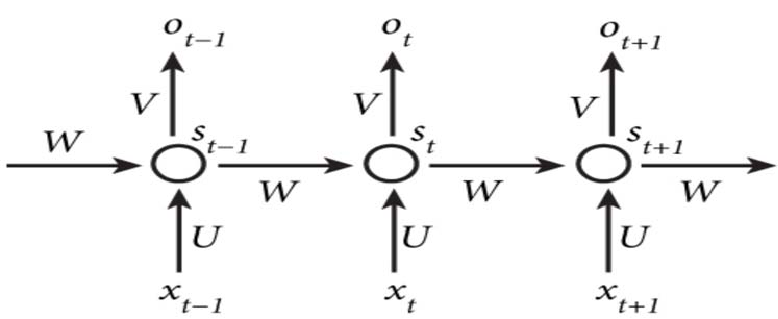
\includegraphics[width=0.9\linewidth]{figs/Background_RNN}
  \caption{Structure of a Recurrent Neural Network consisting of a chain of repeating modules of neural networks. The RNN predicts the next character at each time step $(t+1)$, knowing the history of characters in previous time steps.}
\label{fig:RNN}
\end{figure}
Where \textit{n} represents the number of history words the model uses to predict the next word. Obviously, a higher $n$ results in better prediction, at the cost of higher training time resulting from a more complex model.  

\noindent{\bf Char-RNN-Based Language Modeling}.
Recurrent neural network (RNN) is a very popular class of neural networks for dealing with sequential data, frequently encountered in the NLP domain. The power of RNN is that each neuron or unit can use its internal state memory to save information from the previous input and use that state, together with the current input, to determine what the next output should be. %In this context, we utilize this property to capture long character sequences and relations such as Genome Sequencing with similar way of Language modeling problems in machine learning applications.
Character-level RNN models, \textit{char-RNN} for short, operate by taking a chunk of text and modeling the probability distribution of the next character in the sequence, given a sequence of previous characters. This then allows it to generate new text, one character at a time~\cite{graves2013generating}.
As shown in Fig. \ref{fig:RNN}, RNNs consist of three main layers: Input Layer, Hidden Layer, and Output Layer.
First, Input Layer takes $ x_{t} $ vector, which is input at a time step $t$, usually a one-hot encoding vector of the $ t^{th} $ word or character of the input sentence. 
Second, Hidden Layer consists of the hidden state at the same time step $ s_{t} $, which represents the memory of this network. It is calculated as a non-linear function \textit{f} (\eg tanh ) of the previous hidden state $ s_{t-1} $ and the input at current time step $ x_{t} $ with the following relation: \begin{equation}
s_{t} = f(U x_{t} + W s_{t-1}).
\end{equation}
where, $W$ is a matrix that consists of hidden weights of this hidden layer.
Finally, Output Layer consists of a vector $ o_{t} $, which represents the output at step $t$ and contains prediction probabilities for the next character in the sentence. Formally, its length equals the size of the vocabulary and is calculated using a softmax function.
%\begin{equation}\label{eq:3}
%o_{t} = \mathrm{softmax}(V s_t).
%\end{equation}
% SB (1/28/18): The above equation is a CFC (Candidate For Chop). Softmax is just one of several possibilities. Plus we do not really use this equation in our text later. 
% Mustafa(1/28): done
Backpropagation was used to train the RNN to update weights and minimize the error between the observed and the estimated next word. For Deep RNN architectures, there are multiple parameters that affect the performance of the model. The two main parameters are: \textit{Number of Hidden Layers} and \textit{Number of Neurons per Layer}. For Char-RNN language modeling, vocabulary would include the four nucleotide bases as characters {A, C, G, and T}. Each input is a one-hot encoding vector for the four nucleotides.
% SB (1/28/18): Do we mean ``Each input is a one-hot encoding vector ...''. 
% Mustafa(1/28): done
Each output vector at each time step also has the same dimension.  

\noindent{\bf Perplexity of the Language Model}. 
Perplexity is a measurement of how well a probability distribution predicts a sample. In NLP, perplexity is one of the most effective ways of evaluating the goodness of fit of a language model since a language model is a probability distribution over entire sentences of text~\cite{azzopardi2003investigating}. For example, 5 per word perplexity of a model translates to the model being as confused on test data as if it had to select uniformly and independently from 5 possibilities for each word. Thus, a lower perplexity indicates that language model is better at making predictions.
For an N-Gram language model, perplexity of a sentence is the inverse probability of
the test set, normalized by the number of words. It is clear from \eqref{eq:4} that minimizing perplexity is the same as maximizing the probability of the observed set of $m$ words from $W_{1}$ to $W_{m}$.

\begin{equation}\label{eq:4}
\begin{aligned}
PP(W) &= \sqrt[m]{\frac{1}{P(W_{1},W_{2},....,W_{m})}}\\
&\approx \sqrt[m]{\frac{1}{\displaystyle \prod_{i=1}^{m}P(W_{i} | W_{i-1},...,W_{i-n})}}
\end{aligned}
\end{equation}
For RNN, perplexity is measured as the exponential of the mean of the cross-entropy loss (CE), given by:
\begin{equation}
\begin{aligned}
CE(y, \hat{y}) = - \sum_{i=1}^{|V|} y_{i}\log(\hat{y_i}),
\end{aligned}
\end{equation}
Where $\hat{y}$ is the predicted next character, the output of the RNN, and $|V|$ is the vocabulary size used during training. 

\section{Our Solution: {\bf \name}}
%\SCcomment{So how has previous work chosen best parameters for error correction prior to de novo assembly?} 
%\AMcomment{Addressed in intro. in the paragraph starting with "Many  existing  solutions"}
\subsection{Intuition for the Use of the Perplexity Metric}
Our design uses the Perplexity metric to provide an accurate, and importantly quick, estimation of the quality of error correction with the current configuration parameter value. %\name is useful for both \textit{de novo} assembly where a reference genome is not available and also for comparative sequencing where a reference genome is available but it is expensive to perform the alignment and then calculate the assembly quality to determine the optimal value of configuration parameter.
The perplexity metric is based on using a language model trained on the entire original read set before error correction.
% SB (11/4/18): We are not consistent in the casing ``Perplexity Metric'' ``Perplexity metric'' and ``perplexity metric''. Be consistent. I do not have a strong opinion, but mildly prefer the second one. 
%\SCcomment{explain the intuition for using the perplexity metric on the original uncorrected data, it is a sub-sample of the uncorrected data, right? if so, say how you sub-sample}
%\AMcomment{Language model is trained on original uncorrected data but perplexity is calculated on a sub-sample of corrected reads, we use a sample of 50K/10M reads on RNN.}
The perplexity metric measures how well a learned LM can predict the next element in an input stream. Suppose the input stream is $H$ and the next element is $e$. Then, the perplexity metric is inversely proportional to the probability of seeing ``e'' in the stream, given the history $H$ for the learned model.
This method works because there is a high negative correlation of the perplexity metric with both EC metrics---Alignment Rate and EC Gain.
Given this anti-correlation, we can rely on the perplexity metric as an evaluation function, and apply a simple search technique (\textit{e.g.}, hill climbing) to find the best $k$-value for a given dataset. In this description, for simplicity of exposition, we use the $k$-value in $k$-mer based techniques as an example of \name-tuned configuration parameter. However, \name can tune any other relevant configuration parameter in error correction algorithms and we experimentally show the behavior with another parameter in the RACER tool. 
Figure \ref{fig:PPL_Simple_Example} shows an example how perplexity can evaluate the likelihood of a sequence of $k$-mers using their frequencies and contextual dependencies. In this example, we notice that the corrected read set (\ie on the right) has a considerably lower perplexity value (15.2), relative to the erroneous set (77.72). This is an example of our intuition that the perplexity metric reflects the correctness of the read dataset is validated through a negative relationship.

% SB (11/4/18): Worked till here.

\subsection{Application of Language Models}
We investigate the validity of our approach by training 2 LM variants: 
\begin{enumerate}
\item \textbf{N-Gram Language Models}: Using the SRILM toolkit~\cite{Stolcke02srilm--}, we train an N-Gram model, which is word-based, from the input set of reads before correction. This N-Gram model needs word-segmentation of the input read as a preprocessing phase. Then, we use this trained LM to evaluate the quality of reads after error correction. SRILM is an open source toolkit that supports building statistical N-Gram LMs, in addition to evaluating the likelihood of new sequences using the perplexity metric. 
%\SCcomment{likelihood of new sequences, you mean?}
% Mus: Done.

\item \textbf{RNN Language Models}: The second technique is RNN-based, using different RNN architectures, \eg standard RNNs, LSTMs, and GRUs.
These models can be trained either as word-based models or character-based models. We train them as character-based models to avoid segmentation as a preprocessing phase, in contrast to N-Gram models. We build over the TensorFlow platform for our implementation \cite{45381}.
%\SCcomment{is it just using TensorFlow's N-gram model or do we implement something on top that we can release. This community likes new open-source implementations.}
%\AMcomment{We can open-source \name itself after acceptance}
\end{enumerate}

\noindent{Although N-Gram LMs are much faster compared to RNN-based models, they still have the requirement of splitting a read into words of specific length.}
%\SCcomment{is this pre-processing phase time-consuming or what is the exact problem, specify.}
%\AMcomment{This phase is not time consuming at all, but deciding the word length is somewhat related to finding the k-mer size (see section 3.1 in "A careful reader")} ok
Further, RNN-based models have much lower memory footprint and storage requirements relative to N-Gram. This is because N-Gram models need to store conditional probabilities in large tables (average size of 0.6-1.1 GB across the 5 datasets), while RNNs only need to store the network architecture and  weights (average size of 3-5 MB across the 5 datasets). 
%\SCcomment{remember to fill out the XXX}
% SB (1/28/18): We do not say how we break this circular problem. That can be mentioned here or just above when we introduced the N-gram based model.
From our results, we see that both \name variants efficiently guide the EC algorithm toward selecting the most appropriate configuration parameters (\eg $k$). 

\subsection{Search through the Parameter Space}
Our objective is to find the best $k$-value that will minimize the perplexity of the corrected dataset. We assume that perplexity can be modeled by the following function.
\begin{equation}
Perplexity = f_{n}(LM, D_0, k)
\end{equation} 
Where LM: trained language model, $D_0$: corrected genomic dataset ($S'_c$ in Figure 1), and $k$: the configuration parameter we wish to tune.
$f_{n}$ is a discrete function as values of $k$ are discrete and the derivative of this function is unknown. Therefore, a gradient-based optimization technique will not work. Therefore, we use a simple hill-climbing technique to find the value of $k$ that gives the minimum value of $f_n$, for the given LM and $D_0$.

The following pseudo-code describes the steps used for finding the best $k$-value for a given dataset. We begin by training a language model on the original uncorrected read set ($D_o$). Second, we assume that the best value of $k$ lies in a range from $A$ to $B$ (initially set to either the tool's recommended range, or between 1 and $L$, where $L$ is the read size).
% SB (1/28/18): What is L?
We apply an existing EC algorithm (\eg Lighter or Blue) with different initial values $(k_{0}$,..., $k_{m}) \in (A, B)$, to avoid getting stuck in local minima, going through multiple iterations for a given initial value. We evaluate the perplexity for the corrected dataset with current value of $k$ and its neighbors ($k+\delta$ and $k-\delta$). In each iteration, we apply hill-climbing search to identify the next best value of $k_{i}$ for the following iteration. The algorithm terminates whenever the perplexity relative to $k_i$ is less than the perplexities of both its neighbors or the maximum number of (user-defined) iterations is reached. However, all shown results are with respect to only one initial value (\textit{i.e.}, one iteration). This is intended to show the EC gain of just one iteration, achieving performance within 0.27\% of an exhaustive search across the whole range of $k$ values. %Also with many iterations the solution becomes similar to exhaustive searching.   
%range under investigation is smaller than a user defined value $\alpha$ (set to 1 by default).
% SB (1/28/18): When do we sub-sample? I would imagine we sub-sample before we apply the error correction algorithm, otherwise it will take too long. 
%\SCcomment{use small font for algo}.


\begin{minipage}[t]{.45\textwidth}
%\begin{table}
\begin{algorithm}[H]
\caption{Correct Set of Reads}
\begin{algorithmic} 
\REQUIRE Dataset: $D_{0}$, Read Length: $L$, Maximum number of iterations: $IterMax$
\ENSURE $Corrected Dataset: D_c$
\begin{enumerate}
\itemsep0em
\item Train a Language Model (LM) using $D_{0}$.
\item Select random sample $S'$ from original dataset $D_{0}$.
\item Pick $k_0$,$k_1$,...,$k_m$: initial values of $k$ in the range of (1, L).
\item for i in the range (0, m) 
\item \quad Call \textbf{Find Optimal $K_i$}($S'$, L, LM, IterMax, $k_i$)
\item Take $k$ as the argmin of $K_i$ values picked at step 5 and do a complete correction on the whole dataset.
\end{enumerate}
\end{algorithmic}
\end{algorithm}
\end{minipage}
\hfill
\begin{minipage}[t]{.45\textwidth}
\begin{algorithm} [H]
\caption{Find Optimal $k$}
\begin{algorithmic} 
\REQUIRE Data set: $S'$, Read Length: L, Language Model: LM, MaxNumOfIterations: IterMax, Initial value of $k$: $k_i$ 
%Range start: S, Range end: E
\ENSURE $Best k: k*$
%\scalebox{0.85}{
\begin{enumerate}
\itemsep0em
\item %For k in $\frac{L}{4}, \frac{L}{2}, \frac{3L}{4}$ Do: 
Evaluate perplexity of $k_i$ and its neighbors.
\item If perplexity of $k_i$ is less than perplexities of both its neighbors, return $k_i$ as $k*$
\item Else, set $k_{i+1}$ = value of neighbor with least perplexity.
  % SB (1/28/18): The above is not correct - should be a function of S and E. 
%\item \quad Correct $D_o$ with K-mer = k, save in $D_k$
  % SB (1/28/18): Correct the whole dataset or a sub sample of it?
%\item \quad Select a random sample from $D_k$ and calculate the perplexity of that sample
%\item select the 2 values of k with minimum perplexity, save as A \& B
\item if $i \leq$ IterMax Do:
\item \quad Increment $i$ and Call \textbf{Find Optimal K} ($D_{0}$, L, LM, A, B, $\alpha$, $k_{i+1}$)
\item else  \quad return best $k_i$ so far
\end{enumerate}%}
\end{algorithmic}
\end{algorithm}

\end{minipage}

% \subsection{Time and Space Complexity}
% Because we apply hill climbing search to find the best value of $k$, the worst-case time complexity of the proposed algorithm is linear in terms of the read length. For the space complexity, \name only needs to save the perplexity values of previously investigated values of $k$, which is also linear in terms of the read length.

%As we depend on a simple hill climbing search technique, assuming that the function 
% SB (1/28/18): Give the running time and the memory complexity of our overall algorithm.
% SB (1/28/18): What is the typical number of steps till termination?


\vspace{-5pt}
\section{Evaluation with Real Datasets}
\label{sec:evaluation-real}

In this section, we evaluate \name variants separately by correcting errors in 5 real datasets and evaluating the quality of the resultant assembly. We implement the N-Gram model using the SRILM toolkit~\cite{Stolcke02srilm--}. SRILM is an open source toolkit that supports building statistical N-Gram LMs, in addition to evaluating the likelihood of new sequences using the perplexity metric. For the RNN LM implementation, we build on the TensorFlow platform \cite{45381}.
% SB (11/4/18): Say one sentence more on the RNN implementation/setup that we do. 
After correction, we run the Bowtie2 aligner \cite{langmead2012fast} and measure the Alignment Rate and the Error Correction Gain. A higher value for either metric (i.e., Alignment Rate or Correction Gain) implies superior error correction.
% SB (11/4/18): Space permitting give a one sentence description of what each metric means. 
% Mus(11/5/18): Done.
We do a sweep through a range of $k$-values and measure the alignment rate to determine if the \name-generated $k$-value is optimal or its distance from optimality. For interpreting the execution time results, our experiments were performed on Dell Precision T3500 Workstation, with 8 CPU cores, each running at 3.2GHZ, 12GB RAM, and Ubuntu 16.04 Operating System.
We use 3 EC tools, in pipeline mode with \name, namely, Lighter, Blue, and RACER. Blue uses a k-mer consensus to target different kinds of errors such as substitution, deletion and insertion errors, as well as uncalled bases. This improves the performance of both alignment and assembly \cite{greenfield2014blue}. On the other hand, Lighter is much faster as it uses only a sample of k-mers to perform correction. %\SCcomment{what kinds?}
%Blue is memory efficient and runs faster on large data sets than comparable tools.
Third, RACER uses a different configuration parameter than the value of $k$ and we are able to tune that as well. Specifically, RACER uses the genome length to automatically calculate multiple $k$-values to use for correction.
% SB (11/4/18): Try to play up our strength here - RACER uses a different configuration parameter than the value of k and we are able to tune that as well. Above sentence detracts from our generality story. 
% Mus(11/5/18): Added suggested sentence. Please check.
%\SCcomment{where you say they target different kinds of errors, which one targets what type. Also, how can you tune GL, isn't GL fixed for a genome?}
Our ability to tune any of these EC algorithm's parameters is in line with our vision and ongoing work to design extensible blocks of software to expedite algorithmic development in bioinformatics~\cite{mahadik2016sarvavid}.
Incidentally, we started using another popular EC tool, Reptile, but it only allowed for a smaller range of $k$-values, beyond which it ran into out-of-memory errors. Hence, to demonstrate results with the full range of $k$ values, we restricted our pipelining to Lighter and Blue. 

Our datasets are Illumina short reads [Table \ref{tbl:Datasets_Description}], used in multiple prior studies (\eg~\cite{yang2010reptile, doi:10.1093/bioinformatics/btp379}). For these, there exist ground-truth reference genomes, which we use to evaluate the EC quality. %The first two datasets are Illumina reads from \textit{E. coli}. 
The five datasets have different read lengths (from 36bp in D1\&D3 to 100pb in D5) and different error rates (from $<$ 3\% in D1 to 43\% in D2).  
%The second dataset ``D2'' has higher error rates compared to the first one ``D1". The third dataset ``D3'' has middle-of-the-pack error rates. %``D4'' is from \textit{Bacillus subtilis} with higher read length bp =75. The fifth dataset ``D5'' is from \textit{L. interrogans C} with the highest read length of bp=100.  % and with length of about 47 for each short read (i.e., bp = 47).
% SB (1/28/18): Say which data set is which, what are their error characteristics. % Mus: done
%\SCcomment{skype comment 11:59AM.. basically don't add superfluous info that is already in the table.. talk about the error profiles.}

\begin{table}[H]
\begin{center}
\caption {Datasets' description with coverage, number of reads, length of each read, and the reference genome.} 
\label{tbl:Datasets_Description}
% \begin{adjustbox}{\textwidth}
\small 
\scalebox{0.86}{
 \begin{tabular}{|c|c|c|c|c|c|c|c|} 
 \hline
 Dataset &  Coverage & \#Reads & Read Length & Genome Type & Reference Genome & Accession Number \\ [0.5ex] 
 \hline
 \multirowcell{1}{D1} & 80X & 20.8M &  \multirowcell{1}{36 bp} & \multirowcell{1}{\textit{E. coli} str. K-12 substr} & NC\_000913  & SRR001665 \\
 \hline
 D2 & 71X & 7.1M & 47 bp & \multirowcell{1}{\textit{E. coli} str. K-12 substr} & NC\_000913 & SRR022918  \\ 
 \hline
 D3 & 173X & 18.1M & 36 bp & \multirowcell{1}{\textit{Acinetobacter} sp. ADP1} & NC\_005966 & SRR006332   \\ 
  \hline
  D4 & 62X & 3.5M & 75 bp & \multirowcell{1}{\textit{B. subtilis}} & NC\_000964.3 & DRR000852  \\
   \hline
  D5 & 166X & 7.1M & 100 bp & \multirowcell{1}{\textit{L. interrogans C} sp. ADP1} & NC\_005823.1 & SRR397962    \\
 \hline
\end{tabular}
}
%\end{adjustbox}
\end{center}
\end{table}

\vspace{-12pt}
\subsection{Optimal Parameter Selection}
\vspace{-8pt}
The results of using \name with Lighter, Blue, and RACER tools are shown in Table \ref{tb1:Lighter-Blue-Racer-Perplexity-vs-Alignment} for each dataset. In the third column, the value of $k$ (or, GL for RACER) in bold is the one that gives the best assembly quality, evaluated using ground truth.
% SB (11/4/18): The above sentence will change based on restructuring of the table according to my comment in the table. 
We see that this almost always corresponds to the lowest perplexity scores computed using \name's language modeling (Table \ref{tb1:Lighter-vs-Blue-vs-Racer-Perplexity-vs-Alignment}). %(values in bold in the 4th and 5th columns for RNN and N-gram models). 
% SB (11/4/18): But the reader cannot see because the table does not show it. If true, then say (not shown in the table). 
% Mus(11/5/18): It is on Large Table on Appendix. I referred to that Table.
In the cases where the lowest perplexity does not correspond to the best assembly quality (this happens in 3 of the 10 cases aggregated between Lighter and Blue), the difference in overall alignment rate is small, less than 0.27\% in the worst case.  
%\SCcomment{assembly quality of overall alignment rate?}
Further, the anti-correlation between perplexity and alignment rate holds for both optimal and non-optimal $k$-values. 
%\SCcomment{it said assembly quality, I changed to alignment rate. I don't think you measured assembly quality downstream?}
This shows that our hypothesis is valid across a range of $k$-values. We notice that the feasible range of $k$-values in Blue is (20, 32), distinct from Lighter's. Another interesting observation is that the optimal $k$-values are different across the two different EC tools, Lighter and Blue, for the same dataset, as observed before~\cite{song2014lighter}). 
\name can be applied to a different configuration parameter, GL for the RACER tool, in line with our design as a general-purpose tuning tool.

% For Lighter correction tool, results in this section show the very high correlation between the best value of $k$ used for correction and the corresponding language model perplexity of the data. This strong correlation in Char-based RNN LM perplexity and the best value of $k$ is shown for all data sets as shown in \ref{tb1: Lighter:Perplexity Vs Alignment}. 
% SB (1/28/18): Where is the result here? This is a super important result that is missing. We need to show that the value of K chosen by our algorithm leads to the best alignment.
% Mus: done, I have mentioned Table 2 lighter results.
% \subsection{RNN versus LSTM Sequential Models}
% We trained an RNN language model and Long Short Term Memory (LSTM) model with the same number of hidden layers and number of neurons per layer to compare the performance between them. This was done since LSTM is considered the state-of-the-art model in NLP applications. First, we find that the time for training an LSTM is so much longer than an RNN that it is likely infeasible to be used for our problem statement. 
% % SB (1/28/18): How much longer?
% % Mus: I gave example for one epoch time in both RNN- LSTM
% An LSTM epoch is 3 times longer than an RNN epoch (about 12 hours compared to 4 hours) and convergence for one experimental setup takes 5 epochs.
% Second, we find that the accuracy improvement with LSTM is not significant over RNN. For example, on the validation data set, it gives only a 9\% perplexity improvement over RNN. This is shown in Table \ref{tb:LSTM Vs RNN}. 
% As a result, we continue using RNN as our language model. 
% % SB (1/28/18): We have not introduced earlier the notion of ``sentences'' in our context. 
% % Mus: done

% \begin{table}
% \begin{center}
%  \begin{tabular}{|c | c | c|} 
%  \hline
%  Data set & LSTM perplexity  & RNN perplexity  \\ [0.5ex] 
%  \hline
%  D3 & 3.996 & 4.286  \\ 
%  \hline
% \end{tabular}
% \end{center}
% \caption {A comparison of average perplexity on validation data set (\ie, 5\% of D3) using two different trained language models. The small improvement in accuracy of LSTM over RNN does not justify its much longer training and prediction times.}
% \label{tb:LSTM Vs RNN}
% \end{table}

\vspace{-15pt}
\subsection{N-Gram Language Model Results}
\vspace{-5pt}
We start by training an N-Gram language model from the original dataset. We divide each read into smaller segments (words) of length $L_s$ (set to 7 by default). A careful reader may be concerned that selecting the best value of $L_s$ is a difficult problem in itself, of the same order of difficulty as our original problem. Fortunately, this is {\em not} the case and $L_s$ selection turns out to be a much simpler task. From domain knowledge, 
%\SCcomment{just for my information, where did you get the domain knowledge bit?}
we know that if we use $L_s = 4$ or less, the frequencies of the different words will be similar,
% SB (11/4/18): Can you provide the intuition behind the above claim? 
thus reducing the model's discriminatory power, while a large value will mean that the model's memory footprint increases. We find that for a standard desktop-class machine with 32GB of memory, $L_s = 8$ is the maximum that can be accommodated. Further, we find that the model performance is {\em not} very sensitive in the range (5--7), so we end up using $L_s = 7$.
% SB (11/4/18): Why not Ls=5 since that will need less memory?
The same argument holds for selecting a history of words, and we use a tri-gram model (history of 3 words) for all our experiments.
Second, we compare the perplexity metric for datasets corrected with different $k$-values and compare the perplexity metric (without a reference genome) to the alignment rate (using a reference genome). 
We always report the \textit{average perplexity}, which is just the total perplexity averaged across all words.
Our results show a high negative correlation ($\leq$ -0.946) between the two  metrics on the 5 datasets, as shown in Table \ref{tbl:Fiona_5_datasets_Correlation_N_Gram}. %The negative value of the correlation is because of the expected inverse relationship between the perplexity metric and the alignment rate. 
To reiterate, the benefit of using the perplexity metric is that it can be computed without the ground truth and even where a reference genome is available, it is more efficient than aligning to the reference and then computing the alignment rate. 

% SB (11/4/18): Put exhaustive search first. Then for Athena (N-gram) if it is the same as exhaustive search, just say "SAME as Exhaustive". Same for Athena (RNN). This way the reader does not have to pore through 3 sets of numbers and figure out that they are the same. So for Athena columns only give the numbers if they are different.
% SB (11/4/18): Rows 1 and 2 should be flipped. That means "With Athena (N-gram)" Etc should go above "Lighter". 
\begin{table}
\centering
 \caption {Comparison of Lighter, Blue, and RACER using 5 datasets. This is for finding the best $k$-value (GL for RACER) using \name variants \textit{vs.} exhaustive search. We find either the optimal value or within 0.27\% (over Alignment Rate) and within 8.5\% (EC Gain) of the theoretical best (in the worst case), consistent with the reported results by Lighter (Figure 5 in \cite{song2014lighter}). We also notice that for RACER, GL found by \name is within 3\% of the reference GL (except for the RNN model with D5, which still achieves very close performance for both Alignment Rate and EC Gain.)} 
 %\SCcomment{is something wrong here, GL = 20M? ..for d5, racer, rnn}
\scalebox{0.75}{
\small
\begin{tabular}{ |c|c|c|c|c|c|c|c|c|c| } 
\hline
\multicolumn{10}{|c|}{\textbf{Lighter}}\\
\hline
{\textbf{Dataset}} & \multicolumn{3}{c|}{\textbf{With \name (N-gram)}}& \multicolumn{3}{c|}{\textbf{With \name (RNN)}} & \multicolumn{3}{c|}{\makecell{\textbf{Exhaustive Search}}} \\ 
 \hline
 					 & \makecell{\textbf{Selected}\\ \textbf{$k$}} & \makecell{\textbf{Alignment}\\ \textbf{Rate(\%)}}& \textbf{Gain (\%)} & \makecell{\textbf{Selected} \\ \textbf{$k$}} & \makecell{\textbf{Alignment}\\ \textbf{Rate(\%)}}& \textbf{Gain (\%)} & \makecell{\textbf{Selected} \\ \textbf{$k$}} & \makecell{\textbf{Alignment}\\ \textbf{Rate(\%)}}& \textbf{Gain (\%)} 
\\ \hline
 					 \textbf{D1} & \textbf{k=17} & \textbf{98.95}\% & \textbf{96.3}\% & \textbf{k=17} & \textbf{98.95}\% & \textbf{96.3}\%  & \textbf{k=17} & \textbf{98.95}\% & \textbf{96.3}\%
\\ \hline
                          %&  & k = 8 &  204.849 &  121.88 & 56.9\% \\ 
     					  \textbf{D2} & \textbf{k=17} & \textbf{61.15\%} & \textbf{80.1\%} & \textbf{k=17} & \textbf{61.15\%} & \textbf{80.1\%} & k=15 & \textbf{61.42\%} & \textbf{73.8}\% 
\\ \hline
 					      %&  & k = 8 &  200.513 &  52.82 & 72.91\% \\ 
     				 \textbf{D3} & \textbf{k=17} &  \textbf{80.39\%} & \textbf{95.34\%} & \textbf{k=15} & \textbf{80.44\%} & \textbf{86.78 \%} & \textbf{k=15} & \textbf{80.44\%} & \textbf{86.78 \%} 
\\ \hline                        
                        \textbf{D4} & \textbf{k=17} & \textbf{93.95}\% & \textbf{89.87\%} &
                         \textbf{k=17} & \textbf{93.95\%} & \textbf{89.87\%} &
                         \textbf{k=17} & \textbf{93.95\%} & \textbf{89.87\%}
\\ \hline                           
                         \textbf{D5} & \textbf{k=17} & \textbf{92.15\%} & \textbf{81.7\%} & \textbf{k = 25} & \textbf{92.09\%} & \textbf{83.8\%} &
                         \textbf{k=17} & \textbf{92.15}\% & \textbf{81.7\%} \\
  \hline
  \multicolumn{10}{|c|}{\textbf{Blue}}\\
  \hline
 					 \textbf{D1} & \textbf{k=20} & \textbf{99.53}\% & \textbf{99\%} & \textbf{k=25} & \textbf{99.29\%} & \textbf{98.6\%} & \textbf{k=20} & \textbf{99.53}\% & \textbf{99\%}
\\ \hline
                          %&  & k = 8 &  204.849 &  121.88 & 56.9\% \\ 
     					  \textbf{D2} & \textbf{k=20} & \textbf{57.44\%} & \textbf{4.61\%} & \textbf{k=20} & \textbf{57.44\%} & \textbf{4.61\%} & \textbf{k=20} & \textbf{57.44\%} & \textbf{4.61\%} 
\\ \hline
 					      %&  & k = 8 &  200.513 &  52.82 & 72.91\% \\ 
     				 \textbf{D3}  & \textbf{ k=20} & \textbf{84.17\%} & \textbf{99.2\%} & \textbf{k=20} & \textbf{84.17\%} & \textbf{99.2\%} & \textbf{k=20} & \textbf{84.17\%} & \textbf{99.2\%} 
\\ \hline                        
                         \textbf{D4} & \textbf{ k=20} & \textbf{95.31\%} & \textbf{98.5\%} & \textbf{ k=20} & \textbf{95.31\%} & \textbf{98.5\%} & \textbf{ k=20} & \textbf{95.31\%} & \textbf{98.5\%}
\\ \hline                           
                         \textbf{D5} & \textbf{ k=20} & \textbf{92.33\%} & \textbf{88.9\%} & \textbf{ k=20} & \textbf{92.33\%} & \textbf{88.9\%} & \textbf{ k=20} & \textbf{92.33\%} & \textbf{88.9\%}\\
  \hline
  \multicolumn{10}{|c|}{\textbf{RACER}}\\
  \hline
                         \textbf{D1} & \textbf{GL=4.7M} & \textbf{99.26\%} & \textbf{84.8\%} & \textbf{GL=4.7M} & \textbf{99.26\%} & \textbf{84.8\%} & \textbf{GL=4.7M} & \textbf{99.26\%} & \textbf{84.8\%}\\ 
 \hline
                          %&  & k = 8 &  204.849 &  121.88 & 56.9\% \\ 
     					  \textbf{D2} & \textbf{GL=4.7M} & \textbf{81.15\%} & \textbf{92.9\%} & \textbf{GL=4.7M} & \textbf{81.15\%} & \textbf{92.9\%} & \textbf{GL=4.7M} & \textbf{81.15\%} & \textbf{92.9\%}
\\ \hline
 					      %&  & k = 8 &  200.513 &  52.82 & 72.91\% \\ 
     				 \textbf{D3}  & \textbf{GL=3.7M} & \textbf{84.11\%} & \textbf{88.27\%}  & \textbf{GL=3.7M} & \textbf{84.11\%} & \textbf{88.27\%} & \textbf{GL=3.7M} & \textbf{84.11\%} & \textbf{88.27\%}
\\ \hline                        
                         \textbf{D4} & \textbf{GL=4.2M} & \textbf{95.33\%} & \textbf{97\%} & \textbf{GL=4.2M} & \textbf{95.33\%} & \textbf{97\%} & \textbf{GL=4.2M} & \textbf{95.33\%} & \textbf{97\%}
\\ \hline                           
                         \textbf{D5} & \textbf{GL=4.2M} & \textbf{92.29\%} & \textbf{81.63\%} & \textbf{GL=20M} & \textbf{92.28\%} &  \textbf{80.5\%} & \textbf{GL=4.2M} & \textbf{92.29\%} & \textbf{81.63\%}
  \\ \hline 
  \end{tabular}}
\label{tb1:Lighter-Blue-Racer-Perplexity-vs-Alignment}
\end{table}
\vspace{-8pt}
\begin{comment}


\begin{table}[H]
\centering
\begin{tabular}{ |c|c|c| }
\hline
 Dataset & \makecell{Correlation \\ (N-Gram)} & \makecell{Correlation \\ (RNN)}\\ 
 \hline
 D1 &  -0.977 & -0.938 \\ 
 D2 &  -0.981 & -0.969 \\ 
 D3 &  -0.982 & -0.968 \\   
 D4 &  -0.946 & -0.930 \\
 D5 &  -0.970 & -0.962 \\
\hline
\end{tabular}
%\end{center}
\caption {Correlation value between Perplexity of our proposed approaches and Overall Alignment Rate for our five data sets. This demonstrates the strong relationship between the Perplexity Metric and the Overall Alignment Rate.}
\label{tbl:Correlation_N_Gram}
\end{table}
\end{comment}
%\subsection{RRN-based Language Model Results}

% \subsection{\SBcomment{(CFC) Relation between Perplexity and Data Quality}}

% \SBcomment{ Figure \ref{fig:Alignment Rate Vs Perplexity} shows that as the ratio of error in the data increases, the perplexity of the corresponding language model decreases.
% % SB (1/28/18): Editorial style - give the reference to the result table or figure early on in the discussion. 
% For N-Gram based language model, we train three different SRILM language models (one for each of the five data sets under evaluation). We conclude that as the data set has higher error levels (that is, lower alignment rate) (D2 $>$ D3 $>$ D1), the corresponding language model will have higher perplexity. Therefore, there is a strong correlation between our two metrics, justifying the use of our perplexity metric.
% \begin{figure}
%   \includegraphics[width=\linewidth]{Figures/Alignemnt_Rate_new.eps}
%   \caption{Correlation between perplexities and alignment rates for each data set. The left axis represents the Perplexity value whereas the right axis represents the Alignment Rate percentage. We observe smaller values of perplexities correspond to higher values of alignment rates and vice versa, which reflects the amount of errors in each data set before correction.}
%   \label{fig:Alignment Rate Vs Perplexity}
% \end{figure}
% }

\vspace{-8pt}
\subsection{Char-RNN Language Model Results}
% SB (1/28/18): Point [A] - for reference later on for moving some material here. % Mus: done
For training our RNN, we used the ``tensorflow-char-rnn'' library~\cite{45381}. After parameter tuning, we use the following for our experiments: 2 hidden layers with 300 neurons per layer, output layer with size 4 (i.e., corresponding to the four characters(A,C,G, and T)) mini-batch size, and learning rate of 200 and $2 e^{-3}$ respectively.
% SB (11/4/18): Size of input layer, output layer? 
% Mus(11/5/18): Done.
For each of the 5 datasets, we used 90\% for training, 5\% for validation, and 5\% for testing, with no overlap.
% SB (1/29/18): Did we use k-fold cross validation?
%% We used 2 EC tools, Lighter and Blue, in default mode, with \name automatically tuning $k$, demonstrating \name's extensibility. This is in line with our vision to design extensible blocks of software to expedite algorithmic development~\cite{mahadik2016sarvavid}. 
% SB (1/28/18): We should say what error correction algorithm we are using as default. We need to justify why we use Blue and Lighter but not Reptile. 
% SB (1/28/18): Begin repeat. 
%The main insight from our experiments is that the better version of data set after correction (i.e., where all reads of a data set after correction have higher alignment accuracy with the reference genome) is equivalent to lower perplexity of the language model. For most of existing correcting techniques, the existence of a reference genome is a must to evaluate the strength of such correction. Consequently, one strength of our proposal is that we train the language model on erroneous data (i.e., data set before doing correction) and find that that the language model captures dependencies between characters and mutual information. As a result, the perplexity of the language model on the corrected version of each data set is lower than the erroneous version of the data set.
% SB (1/28/18): End repeat.
% SB (1/28/18): The repeated material from above can be chopped.
% Mus: done

For our char-RNN results, we find that the perplexity metric has a strong negative relation to the overall alignment rate [Table \ref{tbl:Fiona_5_datasets_Correlation_N_Gram}], with the absolute value of the correlation always greater than 0.93.
Here we have to sample the uncorrected set for calculating the perplexity measure because using an RNN to perform the calculation is expensive. This is because it involves, for predicting each character, doing 4 feed-forward passes (corresponding to the one-hot encodings for A, T, G, or C), each through 600 neurons. Empirically, for a test sample size of 50K, this translates to approximately 30 minutes on a desktop-class machine.  
In the experiments with the real datasets, we use $50K$ samples with uniform sampling, and in synthetic experiments, we use $100K$ samples (i.e., only 1\% of the dataset).
%\SCcomment{what fraction of the dataset is this?}.
% We find that the perplexity difference increases roughly linearly with the dataset size.
We find that the perplexity score decreases roughly linearly with increasing dataset size.
% SB (11/4/18): I reworded the above sentence. Verify.
More importantly though, the strong quantitative relationship between perplexity and the EC quality is maintained throughout.
% For D1, the perplexity difference before and after EC is the lowest, with D1 containing the least errors to start with. 

% \begin{table}
% \begin{center}
% \begin{tabular}{ |c|c|c|c| } 
% \hline
% Dataset & K & perplexity & overall alignment rate \\ 
%  \hline
%  D1 & 8 &  103.0057 & 97.45\% \\ 
%  D1 &10 &  103.0057 & 97.45\% \\ 
%  D1 &15 &  103.0048 & 98.83\% \\ 
%  D1 &\textbf{17} &  \textbf{103.00427} & \textbf{98.95}\% \\ 
%  D1 & 25 &  103.00551 & 97.98\% \\ 
%   \hline
%  D2 & 8 &  102.44905 & 56.9\% \\ 
%  D2 & 10 & 102.44905 & 56.9\% \\ 
%  D2 & \textbf{15} & 102.415 & \textbf{61.42\%} \\ 
%  D2 & 17 &  \textbf{102.4134} & 61.15\%\% \\ 
%  D2 & 25 & 102.4254 & 59.19\% \\ 
%   \hline
%  D3  & 8 &  100.32177 & 72.91\% \\ 
%  D3  & 10 & 100.32177 & 72.91\% \\ 
%  D3  & \textbf{15} & \textbf{100.24861} & \textbf{80.44\%} \\ 
%  D3  & 17 & 100.27819 & 80.39\%\% \\ 
%  D3  & 25 & 100.31065 & 75.33\% \\ 
%  \hline
% \end{tabular}
% \end{center}
% \caption {Char-RNN: LM Perplexity vs. Alignment rate}
% \end{table}

% \begin{table}
% \begin{center}
%  \begin{tabular}{|c | c | c|} 
%  \hline
%  Data set & Before Correction & After Correction  \\ [0.5ex] 
%  \hline
%  D1 & 103.006 &  \textbf{103.004} \\ 
%  \hline
%  D2 & 204.849 & \textbf{204.76}  \\
%  \hline
%  D3 & 200.530 & \textbf{200.432}  \\ 
%  \hline
%  D4 & 207.294 & \textbf{204.899}  \\ 
%  \hline
%  D5 & 193.121 & \textbf{193.052}  \\ 
%  \hline
% \end{tabular}
% \end{center}
% \caption {A comparison of the Perplexity metric of 50K samples from short reads before and after doing correction, using Lighter and our Char-RNN Language model. The perplexity is always lower after doing correction compared to before correction.}
% \label{tab: before_after_rnn table}
% \end{table}

\begin{table}[H]
\centering
\caption {Comparison of Overall Alignment Rate between Fiona's and RACER's (with and without \name's tuning). Columns 5 \& 6 demonstrate the strong anti-correlation values between Perplexity and Alignment Rate. The last two columns show the assembly quality (in terms of NG50) before and after correction by Racer tuned with \name. Improvements in NG50 are shown between  parentheses}
% SB (11/4/18): Move the correlation columns first. Put double lines to group columns (e.g., the two correlation columns). 
\scalebox{0.8}{
\begin{tabular}{ |c|c|c|c|c|c|c|c| }
\hline
\makecell{Dataset} & \makecell{Fiona \\ + Bowtie2 \\ (Alignment Rate)} & \makecell{RACER \\ w/o \name \\ + Bowtie2 \\ (Alignment Rate)} & \makecell{RACER \\ w/ \name \\ + Bowtie2 \\ (Alignment Rate)}& \makecell{Correlation \\ (N-Gram)} & \makecell{Correlation \\ (RNN)} & \makecell{NG50 \\ of Velvet \\ w/o EC} & \makecell{NG50 \\ of Velvet \\ w/ (Racer+\name)} \\ 
\hline
D1 &  99.25\% & 85.01\% & \textbf{99.26}\% &  -0.977 & -0.938 & 3019 & 6827 (2.26X)\\
D2 &  73.75\% & 58.66\% & \textbf{81.15}\%&  -0.981 & -0.969 & 47 & 2164 (46X) \\
D3 &  83.12\% & 80.79\% & \textbf{84.11}\% &  -0.982 & -0.968 & 1042 & 4164 (4X) \\
D4 &  95.33\% & 93.86\% &	95.33\% &  -0.946 & -0.930 & 118 & 858 (7.27X) \\
D5 &  \textbf{92.34}\% & 90.91\% &	92.29\% &  -0.970 & -0.962 & 186 & 2799 (15X) \\
\hline
\end{tabular}}
\label{tbl:Fiona_5_datasets_Correlation_N_Gram}
\end{table}

\vspace{-12pt}
\subsection{Comparison with Self-tuning EC Tool}
\vspace{-5pt}
Here, we compare \name with the EC tool, Fiona \cite{schulz2014fiona}, which estimates parameters automatically.
% SB (11/4/18): Does it estimate one or multiple parameters? Are these similar to the parameters that we tune automatically in \name?
The purpose of this comparison is to show that \name can tune $k$-mer-based approaches (RACER specifically for this experiment) to achieve comparable performance to suffix array-based approaches (\eg Fiona), reducing the gap between the two approaches.
% SB (11/4/18): The above hints that suffix array-based approaches are better at EC than k-mer based approaches. 
\cite{yang2012survey} and \cite{molnar2014correcting} show a similar comparison between different EC approaches concluding that the automatic selection of configuration parameters, based on the datasets, is crucial for EC performance.
% SB (11/4/18): However, they do not perform such parameter tuning automatically. Verify and then add in. 
 Table \ref{tbl:Fiona_5_datasets_Correlation_N_Gram} presents the overall alignment rate for our 5 evaluation datasets, calculated after doing correction by Fiona. We notice that RACER, when tuned with \name, outperforms automatic tuning by Fiona in 3 of the 5 datasets, while they were equal in one dataset. Finally, Fiona is only better on $D_{5} $ by $0.05\%$, which may be deemed insignificant.  


\vspace{-12pt}
\subsection{Impact on Assembly Quality}
\vspace{-5pt}

Here we show the impact of tuning EC tools on genome assembly quality. We use Velvet \cite{zerbino2008velvet} to perform the assembly and QUAST \cite{gurevich2013quast} to evaluate the assembly quality. We compare the NG50 before and after correction done by RACER using the best GL found by \name. The results (Table \ref{tbl:Fiona_5_datasets_Correlation_N_Gram}) show a significant improvement on NG50 by 2.26X, 46X, 4X, 7.27X, and 15X. For D1, the improvement in NG50 before and after EC is the lowest, since D1 contains the least fraction of errors to start with. 
These improvements are consistent with what was reported in \cite{heydari2017evaluation} and \cite{greenfield2014blue}. In these prior works, improvement in genomic assembly was measured due to the use of error correction tools
% (same as ours or different?)
with manually tuned configuration parameters.
% SB (11/4/18): Verify above sentence.


\vspace{-5pt}
\subsection{Search time improvement with \name}
\vspace{-5pt}
% SB (1/28/18): I don't understand this. Need to rewrite after sitting down and understanding. 
% This includes time to run for different k values? But this says "average runtime for evaluating
% the quality of correction using N-Gram language model versus the average
% runtime of performing alignment (using Bowtie2 tool [14]).
% This seems to me to be comparing apples and oranges. 

\begin{table}[h]
\centering
\caption {Search time comparison for estimating the perplexity metric with \name (N-gram) for a point in search space \textit{vs}. estimating overall alignment rate with Bowtie2 }%6.2X, 4.8X, 4.7X, 3.6X, and 5.82X, improvements, respectively.}
\scalebox{0.83}{
\begin{tabular}{ |c|c|c|c|c|c|c|c|c|c| }
\hline
\multicolumn{10}{|c|}{\textbf{Dataset}}\\
\hline
 \multicolumn{2}{|c|}{\textbf{D1}} & \multicolumn{2}{|c|}{\textbf{D2}} & \multicolumn{2}{|c|}{\textbf{D3}} & \multicolumn{2}{|c|}{\textbf{D4}} & \multicolumn{2}{|c|}{\textbf{D5}}\\
  \hline
Athena & Bowtie2 & Athena & Bowtie2 & Athena & Bowtie2 & Athena & Bowtie2 & Athena & Bowtie2 \\ 
 \hline
1m 38s & 10m 5s  &  49s & 3m 53s &  1m 39s & 7m 50s &  52s & 3m 8s &  1m 40s & 9m 42s\\ 
 \hline
\end{tabular}}
%\end{center}
\label{tbl:N_Gram_Run_Time_Vs_Bowtie}
\end{table}

Consider that in our problem statement, we are trying to search through a space of configuration parameters in order to optimize a metric (EC Gain or Alignment Rate). The search space can be large and since the cost of searching shows up as a runtime delay, it is important to reduce the time that it takes to evaluate that metric of each search point. In today's state-of-the-art, to find the best value of a configuration parameter~\cite{chikhi2013informed, mahadik2017scalable}, \eg $k$-value, the method would be to pick a $k$ (a single point in the space), run the EC tool with that value, then perform alignment (with one of several available tools such as Bowtie2), and finally compute the metric (alignment rate or EC gain) for that value. In contrast, with \name, to explore one point in the search space, we run the EC algorithm with the $k$-value, and then compute the perplexity metric, which does not involve the time consuming step of alignment. Here, we evaluate the relative time spent in exploring one point in the search space using \name vis-$\grave{a}$-vis the baseline, the state-of-the-art. The result is shown in Table \ref{tbl:N_Gram_Run_Time_Vs_Bowtie}. For this comparison, the alignment is done by Bowtie2~\cite{langmead2012fast}. We find that using the baseline approach, each step in the search takes respectively 6.2X, 4.8X, and 4.7X, 3.6X, and 5.82X for the 5 datasets respectively. Further, while we use the hill-climbing technique to search through the space, today's baseline methods use exhaustive search, such as in Lighter~\cite{song2014lighter} and thus the end-to-end runtime advantage of \name will be magnified. 
% In this experiment, we demonstrate the advantage of using the perplexity metric in tuning the value of $k$ even in cases where a reference genome exists. We show that using the trained language models can reduce the training time greatly compared to applying the alignment phase for each investigated value of $k$. Table \ref{tbl:N_Gram_Run_Time_Vs_Bowtie} shows the average runtime for evaluating the quality of correction using N-Gram language model versus the average runtime of performing alignment (using Bowtie2  tool \cite{langmead2012fast}). The results show a reduction of 0.16x, 0.21x, and 0.19x for the three data sets described in Table \ref{tbl:N_Gram_Run_Time_Vs_Bowtie}.
% SB (1/28/18): Reduction of 16\%, 21\%, and 19\%?

% SB (1/28/18): All the material in this paragraph should be moved and merged with what we have at point [A] (see above in this section).
% Mus: done

% Therefore, the validation perplexity is computed on unseen data during training. Each epoch has a checkpoint that evaluates the perplexity of the language model over validation data set. We found that about ``5'' epochs are enough to have saturation of perplexity using our validation data set. Finally, we choose the checkpoint, named the best model , with the least perplexity, which gave us the best trained language model.

% \item Compare the error correction performance w.r.t the selected value of K to \textit{KMERGENIE}, which has been proposed in \cite{chikhi2013informed}
% \end{enumerate}



% \begin{table*}
% \begin{center}
% \begin{tabular}{ |c|c|c|c|c|c|c|c| } 
% \hline
%  Data Set & K & perplexity (RNN) & perplexity (N-Gram) & aligned 0 times	& aligned exactly 1 &	aligned $\geq$ 1 & overall alignment rate \\ 
%  \hline
%  %D1 & 10 &  \textbf{206.002} &  126.9572  & 7.17\%	& 6.14\%	& 86.69\% & 89.73\% \\ 
%  D1 & \textbf{20} &  206.033 &  \textbf{16.52} & 0.10\%	& 1.60\%	& 98.30\% & \textbf{99.53}\% \\ 
%  D1 & 25 &  \textbf{206.026} &  16.62 & 0.08\%   & 1.81\%	& 98.10\% & 99.29\% \\ 
%  D1 & 30 &  206.0361 &  16.96 & 0.03\%	& 2.35\% &	97.62\%  & 98.65\% \\ 
%  \hline
%  %D2 & 10 & 204.888 & 168.75 & 5.02\%	& 46.58\%	& 48.40\%  & 55.31\% \\ 
%  D2 & \textbf{20} & \textbf{204.846} & \textbf{119.1738}   & 2.52\%	& 46.00\%  & 51.48\% & \textbf{57.44}\% \\ 
%  D2 & 25 &  204.848 & 120.5232 & 2.39\% & 46.43\% &	51.18\% & 57.09\% \\ 
%  D2 & 30 & 204.847 & 238.98 & 2.35\%	& 46.57\%	& 51.07\%  & 57\% \\ 
%  \hline
%  %D3 & 10 & 200.481 & 100.98 &  31.51 \%	& 67.01\%	& 1.48\% & 68.49\% \\ 
%  D3 & \textbf{20} & \textbf{200.46}  & \textbf{29.89}   & 3.09\%	& 18.47\% &	78.44\% & \textbf{84.17}\% \\ 
%  D3 & 25 & 200.49   & 32.39 & 3.03\%	& 20.59\% &	76.38\% & 81.62\% \\ 
%  D3 & 30 & 200.51 & 49.22 & 2.34\%	& 31.38\%	& 66.28\% & 73.84\% \\
%   \hline
% \end{tabular}
% \end{center}
% \caption {Blue Results for our three data sets: It contains a comparison between finding best value of $k$ using our proposed approaches (i.e., N-Gram and Char-RNN language models perplexities) and finding best value of $k$ using the Alignment Rate metric. For N-Gram column: Sample of test data is the whole reads after correction but for Char-RNN, a sample of $50K$ was used. We notice that Blue differs from Lighter as Blue can align corrected reads more than once with reference genome as the value of $k$ approaches optimal value.}\label{tb1: Blue Results}
% \end{table*}

% \begin{table}
% \begin{center}
%  \begin{tabular}{| c | c |  c |  c |} 
%  \hline
% Data set & Injected Error Type & High rate & Low rate  \\ [0.5ex] 
%  \hline
% D12 & Insertion & 414.989 &  413.469 \\ 
% D12 & Substitution &  414.541& 413.289 \\
% D12 & Deletion & 413.274 & \textbf{412.782}  \\ 
% D12 & Mixed &  413.721 & 412.925  \\ 
%  \hline
% D3 & Insertion & 404.709 &  402.817\\ 
%  D3 & Substitution &  404.273& 402.679 \\
%  D3 & Deletion & 402.541 & \textbf{401.908}  \\ 
%  D3 & Mixed & 403.251 & 402.166  \\ 
%  \hline 
% \end{tabular}
% \end{center}
% \caption {Char-RNN Perplexity metric for different types of synthetic errors: Deletion, Insertion, and Substitution for data sets D12(i.e., both data sets D1 and D2 as they have same reference genome) and D3(It is from a different reference genome). We compare two versions of such errors: High error rate and low error rate.}
% \label{tb1: Char-RNN Synthetic}
% \end{table}
%\SCcomment{why do you think we are better than Fiona? give the intuition.}

\vspace{-12pt}
\section{Related Work}
\vspace{-12pt}
\textbf{Error Correction Approaches:} EC tools can be mainly divided into three categories: $k$-spectrum based, suffix tree/array-based, and multiple sequence alignment-based (MSA) methods. Authors in \cite{pevzner2001eulerian} explained the procedure of using $k$-mers for error correction. %This involved first converting reads with insolid $k$-mers %, \ie, $k$-mers that occurred less than $M$ times in a given sequence dataset, 
%to solid ones with edit distance operations. As a result, the sequence then contains only solid $k$-mers. By identifying such $k$-mer sets, alignment is directly performed. 
While this work and others show that choosing a proper $k$ value results in a satisfactory overall assembly, no data-driven method is provided. Second, Suffix tree/array-based EC tools, \eg \cite{ilie2010hitec}, generalizes the $k$-mer based approach by handling multiple $k$ values and the corresponding threshold $M$. Finally, MSA research presented in \cite{salmela2011correcting} used $k$-mers as seeds and generated an adapted sequence that will be aligned further. Moreover, authors in \cite{chikhi2013informed} proposed an approach for finding the optimal $k$-values for genome assembly. However, the approach doesn't consider the optimal $k$-values for the error correction problem. Moreover, this approach depends on fitting histograms of unique k-mers and for some datasets it is not be able to fit the histogram to the generative model. ECHO \cite{kao2011echo} is an EC tool that doesn't require a user-defined k-mer value, it relies on perfoming multiple correction iterations with different values of $k$. However, only substitutions errors are considered and the runtime of the tool is reported to be very slow for some datasets (in terms of days) \cite{yang2012survey}. % and will not be able to find the best value of $k$. %Moreover, the proposed approach (as it depends on the abundance histograms of unique $k$-mers) cannot be easily adapted for other performance-critical parameters.
%Many open source EC tools are available, \eg Reptile~\cite{yang2010reptile}, Quake~\cite{kelley2010quake}, and PReptile~\cite{shah2012parallel}. All of these software modules measure three main metrics: 1) the accuracy of error correction, 2) runtime, and 3) memory usage. All three metrics can be affected by the selected value of $k$ and hence can be tuned with \name. 
%clarify above.. proposed approach
% Also authors in \cite {yang2012survey}  used ``gain'' metric to judge each system's performance, where gain is defined as the percentage of errors removed from the data set by the error-correction program, and thus requires a reference genome to estimate. However, it is not clear how the evaluation of the quality of correction is estimated in the absence of a reference genome.
\\
\textbf{Language Modeling in Genomics:} In the genomics domain, language modeling was used in \cite{ganapathiraju2002comparative} to find the characteristics of organisms in which N-gram analysis was applied to 44 different bacterial and archaeal genomes and to the human genome. 
% Moreover, \cite{ganapathiraju2012suite} 
In subsequent work, they used N-Gram language modeling for extracting patterns from whole genome sequences. Others~\cite{coin2003enhanced} have used language modeling to enhance domain recognition in protein sequences. For example, \cite{king2007ngloc} has used N-gram analysis specifically to create a Bayesian classifier to predict the localization of a protein sequence over 10 distinct eukaryotic organisms. 
RNNs can be thought of as a generalization of Hidden Markov Models (HMMs) and HMMs have been applied in several studies that seek to annotate epigenetic data. For example, \cite{song2015spectacle} presents a fast method of using spectral learning with HMMs for annotating chromatin states in the human genome.
Thus, we are seeing the use of various ML techniques traditionally used in NLP being used to make sense of biological data.  
\vspace{-5pt}

\vspace{-12pt}
\section{Discussion}
\vspace{-5pt}
A single iteration in \name assumes that the perplexity metric is convex in relation to the value of $k$. Intuitively, with small $k$-values, most $k$-mers will have high frequencies and hence very few will be corrected. In contrast, with high $k$-values, the number of unique $k$-mers increases, and hence no subset of $k$-mers is of high-enough fidelity. Based on the above rationale, we expect \name to perform accurately for most datasets, as hill climbing search reaches optimal solutions for convex problems. However, for non-convex spaces, a single iteration in \name may get stuck in local optima and therefore several iterations (with different intial points) is needed.  Moreover, some EC tools have a number of performance-sensitive configuration parameters, with interdependencies. For such tools, systems such as Rafiki \cite{mahgoub2017rafiki} can encode such dependencies, while relying on \name's LM to compute the corresponding performance metric, converging toward optimal parameters.


\vspace{-12pt}
\section{Conclusion}
\vspace{-6pt}
The performance of most EC tools for NGS reads is highly dependent on the proper choice of its configuration parameters, \eg $k$-value selection in \textit{k}-mer based techniques as shown in Table \ref{tb1:Lighter-Blue-Racer-Perplexity-vs-Alignment}. Using our \name suite, we target the problem of automatically tuning these parameters using language modeling techniques from the NLP domain without the need for a ground truth genome. 
%\SCcomment{say k-mer-based EC tool instead}
Through N-Gram and char-RNN language modeling, we validate the intuition that the EC performance can be computed quantitatively using the ``perplexity'' metric, which then guides a hill climbing-based search toward the best $k$-value. 
We evaluate \name with 5 different real datasets, plus, with synthetically injected errors. We find that the predictive performance of the perplexity metric is maintained under all scenarios, with absolute correlation scores higher than 0.93. Further, using the perplexity metric, \name can search for and arrive at the best $k$-value, or within 0.27\% of the assembly quality obtained using brute force.



%\section{Acknowledgements} 
%This work was supported by a grant by ...

\bibliographystyle{myrecomb}

\bibliography{athena}

\section{Appendix}
\vspace{-5pt}
\subsection{Background}

\noindent{\bf Error Correction and Evaluation} 

The majority of error correction tools share the following intuition: high-fidelity sequences (or, solid sequences) can be used to correct errors in low-fidelity sequences (or, in-solid sequences). However, they vary significantly in the way they differentiate between solid and in-solid sequences. For example, \cite{yang2010reptile} corrects genomic reads containing insolid $k$-mers using a minimum number of edit operations such that these reads contain only solid $k$-mers after correction.
% SB (1/28/18): Give some representative examples here (1-2 sentences). 
% Mustafa(1/28): done
The evaluation of \textit{de novo} sequencing techniques rely on likelihood-based metrics such as ALE and CGAL, without relying on the availability of a reference genome. On the other hand, comparative sequencing or re-sequencing, such as to study structural variations among two genomes, do have reference genomes available. 
% Moreover, the evaluation criteria for error correction techniques also vary based on the availability of a reference genome. For example, metrics such as Sensitivity, Specificity, and Gain, rely on a comparison with the reference genome to estimate the quality of the reads after correction. However, such metrics cannot be used for re-sequencing, where no reference genome is available, or when studying structural variations in known species. This is where \textit{Athena} whereby the use of the modeling perplexity metric removes the need for a reference genome.
% SB (1/28/18): And we do not have this problem. So mention that here. 
% SC (01/28): done

\noindent{\bf Language Modeling}

To increase the accuracy of detecting words in speech recognition, language modeling techniques have been used to see which word combinations have higher likelihood of occurrence than others, thus improving context-based semantics. Thus, language modeling is being used in many applications such as speech recognition, text retrieval, and many NLP applications. The main task of these statistical models is to capture historical information and predict the future sequences based on that information.
% Language models were originally targeted to improve the performance of automated speech recognition systems. However, they also play a critical role in a wide range of NLP problems. 

\noindent{\bf N-Gram-Based Language Modeling}. 
This type of modeling is word-based.
% , which means that each read has to be divided into several segments before we train such a model.
The main task that N-Gram based models \cite{brown1992class} have been used for is to estimate the likelihood of observing a word \textit{$W_i$}, given the set of previous words ${W_0, \cdots W_{i-1}}$, estimated using the following equation:
\newline
\begin{equation}
\begin{aligned}
  P(W_0, W_1, ..., W_{m}) &= \prod_{i=1}^{m}  P(W_{i} |  W_{i-1}, ..., W_{1}) \\
  &\approx \prod_{i=1}^{m}  P(W_{i} |  W_{i-1}, ..., W_{i-n})
  \end{aligned}
\end{equation}
\begin{figure}
  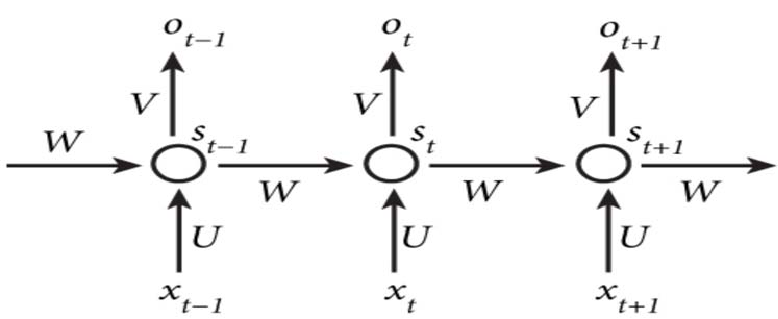
\includegraphics[width=0.9\linewidth]{figs/Background_RNN}
  \caption{Structure of a Recurrent Neural Network consisting of a chain of repeating modules of neural networks. The RNN predicts the next character at each time step $(t+1)$, knowing the history of characters in previous time steps.}
\label{fig:RNN}
\end{figure}
Where \textit{n} represents the number of history words the model uses to predict the next word. Obviously, a higher $n$ results in better prediction, at the cost of higher training time resulting from a more complex model.  

\noindent{\bf Char-RNN-Based Language Modeling}.
Recurrent neural network (RNN) is a very popular class of neural networks for dealing with sequential data, frequently encountered in the NLP domain. The power of RNN is that each neuron or unit can use its internal state memory to save information from the previous input and use that state, together with the current input, to determine what the next output should be. %In this context, we utilize this property to capture long character sequences and relations such as Genome Sequencing with similar way of Language modeling problems in machine learning applications.
Character-level RNN models, \textit{char-RNN} for short, operate by taking a chunk of text and modeling the probability distribution of the next character in the sequence, given a sequence of previous characters. This then allows it to generate new text, one character at a time~\cite{graves2013generating}.
As shown in Fig. \ref{fig:RNN}, RNNs consist of three main layers: Input Layer, Hidden Layer, and Output Layer.
First, Input Layer takes $ x_{t} $ vector, which is input at a time step $t$, usually a one-hot encoding vector of the $ t^{th} $ word or character of the input sentence. 
Second, Hidden Layer consists of the hidden state at the same time step $ s_{t} $, which represents the memory of this network. It is calculated as a non-linear function \textit{f} (\eg tanh ) of the previous hidden state $ s_{t-1} $ and the input at current time step $ x_{t} $ with the following relation: \begin{equation}
s_{t} = f(U x_{t} + W s_{t-1}).
\end{equation}
where, $W$ is a matrix that consists of hidden weights of this hidden layer.
Finally, Output Layer consists of a vector $ o_{t} $, which represents the output at step $t$ and contains prediction probabilities for the next character in the sentence. Formally, its length equals the size of the vocabulary and is calculated using a softmax function.
%\begin{equation}\label{eq:3}
%o_{t} = \mathrm{softmax}(V s_t).
%\end{equation}
% SB (1/28/18): The above equation is a CFC (Candidate For Chop). Softmax is just one of several possibilities. Plus we do not really use this equation in our text later. 
% Mustafa(1/28): done
Backpropagation was used to train the RNN to update weights and minimize the error between the observed and the estimated next word. For Deep RNN architectures, there are multiple parameters that affect the performance of the model. The two main parameters are: \textit{Number of Hidden Layers} and \textit{Number of Neurons per Layer}. For Char-RNN language modeling, vocabulary would include the four nucleotide bases as characters {A, C, G, and T}. Each input is a one-hot encoding vector for the four nucleotides.
% SB (1/28/18): Do we mean ``Each input is a one-hot encoding vector ...''. 
% Mustafa(1/28): done
Each output vector at each time step also has the same dimension.  

\noindent{\bf Perplexity of the Language Model}. 
Perplexity is a measurement of how well a probability distribution predicts a sample. In NLP, perplexity is one of the most effective ways of evaluating the goodness of fit of a language model since a language model is a probability distribution over entire sentences of text~\cite{azzopardi2003investigating}. For example, 5 per word perplexity of a model translates to the model being as confused on test data as if it had to select uniformly and independently from 5 possibilities for each word. Thus, a lower perplexity indicates that language model is better at making predictions.
For an N-Gram language model, perplexity of a sentence is the inverse probability of
the test set, normalized by the number of words. It is clear from \eqref{eq:4} that minimizing perplexity is the same as maximizing the probability of the observed set of $m$ words from $W_{1}$ to $W_{m}$.

\begin{equation}\label{eq:4}
\begin{aligned}
PP(W) &= \sqrt[m]{\frac{1}{P(W_{1},W_{2},....,W_{m})}}\\
&\approx \sqrt[m]{\frac{1}{\displaystyle \prod_{i=1}^{m}P(W_{i} | W_{i-1},...,W_{i-n})}}
\end{aligned}
\end{equation}
For RNN, perplexity is measured as the exponential of the mean of the cross-entropy loss (CE), given by:
\begin{equation}
\begin{aligned}
CE(y, \hat{y}) = - \sum_{i=1}^{|V|} y_{i}\log(\hat{y_i}),
\end{aligned}
\end{equation}
Where $\hat{y}$ is the predicted next character, the output of the RNN, and $|V|$ is the vocabulary size used during training. 

\subsection{Detailed Results}

In this section, we show a detailed version of the results presented in table \ref{tb1:Lighter-Blue-Racer-Perplexity-vs-Alignment}. 
%\begin{comment}
\begin{table}
\centering
7

%\begin{adjustbox}{\textwidth}
\small
\begin{tabular}{ |c|c|c|c|c|c|c| } 
\hline
EC Tool & {Dataset} & Tuned Parameter & \makecell{Perplexity\\(RNN)} & \makecell{Perplexity\\(N-Gram)} & \makecell{Overall Alignment\\ Rate} & Gain (\%) \\  
 \hline
					  %&  & k = 8 & 103.00577 & 20.41 & 97.45\% \\ 
 					  &  & k = 10 & 103.00579 & 20.42 & 97.45\% & -0.01\% \\ 
 					  & D1 & k = 15 & 103.0048 & 16.86 & 98.83\% & 87.5\% \\ 
 					  &  & \textbf{k = 17} & \textbf{103.004} &  \textbf{16.7}  & \textbf{98.95}\% & \textbf{96.3}\% \\ 
 					  &  & k = 25 &  103.00551 &  18.22 & 97.98\% & 69.5\%  
\\\cline{2-7}
                          %&  & k = 8 &  204.849 &  121.88 & 56.9\% \\ 
     					  &  & k = 10 & 204.849 & 121.88 & 56.9\% & 0\%  \\ 
						  & D2 & \textbf{k = 15} & 204.775 & 102.13 & \textbf{61.42\%} & 73.8\% \\ 
     					  &  & k = 17 &  \textbf{204.76} &  \textbf{100.30}  & 61.15\% & \textbf{80.1}\% \\
     					  &  & k = 25 & 204.795 & 107.37 & 59.19\%  & 69.96\%
 \\\cline{2-7}
 					      %&  & k = 8 &  200.513 &  52.82 & 72.91\% \\ 
     		\multirow{4}{*}{Lighter} &  & k = 10 & 200.513 & 52.81 & 72.91\% & 0\% \\ 
     					  & D3 & \textbf{k = 15} & 200.432 & 33.2602 & \textbf{80.44\%} & 86.78 \% \\ 
     					  &  & k = 17 & \textbf{200.432} & \textbf{32.74}  & 80.39\% & \textbf{95.34\%}\\ 
     					  &  & k = 25 & 200.529 & 42.28 & 75.33\% & 65\%
 \\\cline{2-7}                         
                          %&  & k = 8 & 207.2942 & 25.54 & 92.16\% \\
                           &  & k = 10 & 207.2945 & 25.53 & 92.14\% & 0\%\\
                           & D4 & k = 15 & 206.248 & 18.07 & 93.72\% & 86.14 \%\\
                           &  & \textbf{k = 17} & \textbf{204.899} & \textbf{17.86} & \textbf{93.95}\% & 89.87\%\\
                             %& D4 & k-mer Length=20 & 205.634 & 17.86 & 6.31\%	& 91.70\%	& 1.99\% & 93.69\% \\
                             &  & k = 25 & 206.848 & 18.25 &  93.13\% & \textbf{89.9} \%
\\\cline{2-7}                            
                           % &  & k = 8 & 193.121 & 6.44 & 91.92\% \\
                            &  & k = 10 & 193.121 & 6.44 & 91.92\% & 0\%\\
                            & D5 & k = 15 & 193.052 & 5.45 & 92.11\% & 73.12\% \\
                            &  & \textbf{k = 17} & 193.054  &  \textbf{5.354}  & \textbf{92.15}\% & 81.7\% \\
                        %& D5 & k-mer Length=20 & \textbf{193.051} & 5.354 & 7.87\%	& 87.71\%	& 4.42\% & 92.13\% \\    
                 &  & k = 25 & \textbf{193.052} & 5.357 & 92.09\% & \textbf{83.8}\%\\                 
  \hline
  \end{tabular}
%\end{adjustbox}
%\end{center}
\caption {Detailed results for our 5 datasets using Lighter: a comparison between finding best value of $k$ using \name variants vs exhaustive seraching. These results are consistent with the reported results by Lighter's authors (see Figure 5 in \cite{song2014lighter}).}
\label{tb1:Lighter-Perplexity-vs-Alignment}
\end{table}
%\end{comment}

%\begin{comment}

\begin{table}
\centering
%\begin{adjustbox}{\textwidth}
\small
\begin{tabular}{ |c|c|c|c|c|c|c| } 
\hline
EC Tool & {Dataset} & Tuned Parameter & \makecell{Perplexity\\(RNN)} & \makecell{Perplexity\\(N-Gram)} & \makecell{Overall Alignment\\ Rate} & Gain (\%) \\ 
 \hline
						 &  & \textbf{k = 20} &  206.033 &  \textbf{16.52} & \textbf{99.53}\% & \textbf{99\%} \\ 
					   & D1 & k = 25 &  \textbf{206.026} &  16.62 & 99.29\% & 98.6\%\\ 
					   &  & k = 30 &  206.0361 &  16.96 & 98.65\% & 87.6\% 
 \\\cline{2-7}
 %D2 & 10 & 204.888 & 168.75 & 5.02\%	& 46.58\%	& 48.40\%  & 55.31\% \\ 
 \multirow{4}{*}{Blue} &  & \textbf{k = 20} & \textbf{204.846} & \textbf{119.1738} & \textbf{57.44\%} & \textbf{4.61\%} \\ 
 					   & D2 & k = 25 &  204.848 & 120.5232 & 57.09\% & 1.7\% \\ 
 					   &  & k = 30 & 204.847 & 238.98 & 57\%  & 1.24\%  
 \\\cline{2-7}
 %D3 & 10 & 200.481 & 100.98 &  31.51 \%	& 67.01\%	& 1.48\% & 68.49\% \\ 
 					  &  & \textbf{k = 20} & \textbf{200.46}  & \textbf{29.89} & \textbf{84.17}\% & \textbf{99.2\%} \\ 
  					  & D3 & k = 25 & 200.49   & 32.39 & 81.62\% & 97.7\% \\ 
  					  &  & k = 30 & 200.51 & 49.22 & 73.84\% & 13.17 \%
 \\\cline{2-7}                     
%                       & D4 & k-mer Length=15 & 207.155 & 48.18 & 5.70\%	& 92.25\%	& 2.05\% & 94.30\% \\
                        &  & \textbf{k = 20} & \textbf{207.179} & \textbf{46.6} & \textbf{95.31\%} & \textbf{98.5\%} \\
                       & D4 & k = 25 & 207.228 & 47.59 & 94.64\% & 98.4\% \\  
                &  & k = 30 & 207.284 & 48.69 & 93.97\%   & 96.5\%     
                         
%                   & D5 & k-mer Length=15 & 192.785 & 16.16 & 8.01\%	& 87.54\%	& 4.45\% & 91.99\% \\
\\\cline{2-7}
                &  & \textbf{k = 20} & \textbf{192.804} & \textbf{15.67} & \textbf{92.33}\% & 88.9\% \\   
               & D5 & k = 25 & 192.8044 & 15.72 & 92.28\% & \textbf{91.2\%} 
\\               
                &  & k = 30 & 192.8077 & 15.79 & 92.22\%  & 92.08\%
\\           
  \hline
  \end{tabular}
%\end{adjustbox}
%\end{center}
\caption {Detailed results for our 5 datasets using Blue}
\label{tb1:Blue-Perplexity-vs-Alignment}
\end{table}
%\end{comment}

%begin{comment}

\begin{table}
\centering
%\begin{adjustbox}{\textwidth}
\small
\begin{tabular}{ |c|c|c|c|c|c|c| } 
\hline
EC Tool & {Dataset} & Tuned Parameter & \makecell{Perplexity\\(RNN)} & \makecell{Perplexity\\(N-Gram)} & \makecell{Overall Alignment\\ Rate} & Gain(\%) \\ 
 \hline
  %&  & GL = 1M & 206.120 & 45.33 &  85.01\%  & -1253.9\% \\ 
 						 & D1 & \textbf{GL = 4.7M} & \textbf{206.033} & \textbf{16.6} & \textbf{99.26}\% & \textbf{84.8\%} 
 \\ 						  
						 &  & GL = 20M & 206.036 & 16.9 &  98.85\% &  80.3\% \\ 
 						 &  & GL = 30M & 206.0357 & 16.99 & 98.82\% & 77.6\%
 \\\cline{2-7}
   					%	 &  & GL = 1M & 204.839 & 126.16  & 58.66\% & -72.2\% \\
  						 & D2 & \textbf{GL = 4.7M} & \textbf{204.7520} & \textbf{85.14}  & \textbf{81.15}\% & 92.9\% \\
                         &  & GL = 7M & 204.7564 & 85.2  & 81.13\% & \textbf{93\%}\\
                         &  & GL = 30M & 204.775 & 88.24  & 79.24\% & 91.9\%
  \\\cline{2-7}                       
             % &  & GL = 1M & \textbf{200.411} & 56.86  & 71.22\% & -388\% \\
               \multirow{4}{*}{Racer}          &  & \textbf{GL = 3.7M} & 200.4552 & \textbf{30.4}  & \textbf{84.11}\% & 88.27\% \\                                               
                         & D3 & GL = 18M & 200.4603 & 33.87 & 80.97\% & 80.21\% \\
                         &  & GL = 30M & 200.4626 & 34.46  & 80.79\%b & 75.74\%
  \\\cline{2-7}                       
               %          &  & GL = 1M & 206.978 & 19.64 & 93.86\% & 48.3\% \\
                         & D4 & \textbf{GL = 4.2M} & \textbf{206.942} & \textbf{17.32} & \textbf{95.33}\% & \textbf{97\%} \\
                         &  & GL = 20M & 206.9494 & 17.51 & 95.04\% & 96.5\% \\
                         &  & GL = 30M & 206.9489 & 17.53 & 95.01\% & 95.9\%
  \\\cline{2-7}                       
                %         &  & GL = 1M & 193.0461 & 5.46  & 90.91\% & -232.8\% \\
                         
                         & D5 & \textbf{GL = 4.2M} & 193.0454 & \textbf{4.77} & \textbf{92.29}\% & 81.63\%\\
                         &  & GL = 20M & \textbf{193.0451} & 4.78  & 92.28\% & 80.5\% \\
                         &  & GL = 30M & 193.0479 & 4.79  & 92.26\% & 81.9\% \\
  \hline
  \end{tabular}
%\end{adjustbox}%
%\end{center}
\caption {Detailed results for our 5 datasets using Racer.}
\label{tb1:Racer-Perplexity-vs-Alignment}
\end{table}
%\end{comment}

\begin{comment}
\begin{table}
\begin{center}
%\begin{adjustbox}{\textwidth}
\small
\begin{tabular}{ |c|c|c|c|c|c| } 
\hline
EC Tool & {Dataset} & Tuned Parameter & {perplexity (RNN)} & {perplexity (N-Gram)} & {overall alignment rate} \\ 
 \hline
					  %&  & k = 8 & 103.00577 & 20.41 & 97.45\% \\ 
 					  &  & k = 10 & 103.00579 & 20.42 & 97.45\% \\ 
 					  & D1 & k = 15 & 103.0048 & 16.86 & 98.83\% \\ 
 					  &  & \textbf{k = 17} & \textbf{103.004} &  \textbf{16.7}  & \textbf{98.95}\% \\ 
 					  &  & k = 25 &  103.00551 &  18.22 & 97.98\%  
\\\cline{2-6}
                          %&  & k = 8 &  204.849 &  121.88 & 56.9\% \\ 
     					  &  & k = 10 & 204.849 & 121.88 & 56.9\% \\ 
						  & D2 & \textbf{k = 15} & 204.775 & 102.13 & \textbf{61.42\%} \\ 
     					  &  & k = 17 &  \textbf{204.76} &  \textbf{100.30}  & 61.15\% \\
     					  &  & k = 25 & 204.795 & 107.37 & 59.19\% 
 \\\cline{2-6}
 					      %&  & k = 8 &  200.513 &  52.82 & 72.91\% \\ 
     		\multirow{4}{*}{Lighter} &  & k = 10 & 200.513 & 52.81 & 72.91\% \\ 
     					  & D3 & \textbf{k = 15} & \textbf{200.432} & 33.2602 & \textbf{80.44\%} \\ 
     					  &  & k = 17 & 200.432 & \textbf{32.74}  & 80.39\% \\ 
     					  &  & k = 25 & 200.529 & 42.28 & 75.33\% 
 \\\cline{2-6}                         
                          %&  & k = 8 & 207.2942 & 25.54 & 92.16\% \\
                           &  & k = 10 & 207.2945 & 25.53 & 92.14\% \\
                           & D4 & k = 15 & 206.248 & 18.07 & 93.72\% \\
                           &  & \textbf{k = 17} & \textbf{204.899} & \textbf{17.86} & \textbf{93.95}\% \\
                             %& D4 & k-mer Length=20 & 205.634 & 17.86 & 6.31\%	& 91.70\%	& 1.99\% & 93.69\% \\
                             &  & k = 25 & 206.848 & 18.25 &  93.13\% 
\\\cline{2-6}                            
                           % &  & k = 8 & 193.121 & 6.44 & 91.92\% \\
                            &  & k = 10 & 193.121 & 6.44 & 91.92\% \\
                            & D5 & k = 15 & \textbf{193.052} & 5.45 & 92.11\% \\
                            &  & \textbf{k = 17} & 193.054  & \textbf{5.354}  & \textbf{92.15}\% \\
                        %& D5 & k-mer Length=20 & \textbf{193.051} & 5.354 & 7.87\%	& 87.71\%	& 4.42\% & 92.13\% \\    
                 &  & k = 25 & 193.052 & 5.357 & 92.09\% \\                 
  \hline
						 &  & \textbf{k = 20} &  206.033 &  \textbf{16.52} & \textbf{99.53}\% \\ 
					   & D1 & k = 25 &  \textbf{206.026} &  16.62 & 99.29\% \\ 
					   &  & k = 30 &  206.0361 &  16.96 & 98.65\%  
 \\\cline{2-6}
 %D2 & 10 & 204.888 & 168.75 & 5.02\%	& 46.58\%	& 48.40\%  & 55.31\% \\ 
 \multirow{4}{*}{Blue} &  & \textbf{k = 20} & \textbf{204.846} & \textbf{119.1738} & \textbf{57.44}\% \\ 
 					   & D2 & k = 25 &  204.848 & 120.5232 & 57.09\% \\ 
 					   &  & k = 30 & 204.847 & 238.98 & 57\% 
 \\\cline{2-6}
 %D3 & 10 & 200.481 & 100.98 &  31.51 \%	& 67.01\%	& 1.48\% & 68.49\% \\ 
 					  &  & \textbf{k = 20} & \textbf{200.46}  & \textbf{29.89} & \textbf{84.17}\% \\ 
  					  & D3 & k = 25 & 200.49   & 32.39 & 81.62\% \\ 
  					  &  & k = 30 & 200.51 & 49.22 & 73.84\%
 \\\cline{2-6}                     
%                       & D4 & k-mer Length=15 & 207.155 & 48.18 & 5.70\%	& 92.25\%	& 2.05\% & 94.30\% \\
                        &  & \textbf{k = 20} & \textbf{207.179} & \textbf{46.6} & \textbf{95.31}\% \\
                       & D4 & k = 25 & 207.228 & 47.59 & 94.64\% \\  
                &  & k = 30 & 207.284 & 48.69 & 93.97\%       
                         
%                   & D5 & k-mer Length=15 & 192.785 & 16.16 & 8.01\%	& 87.54\%	& 4.45\% & 91.99\% \\
\\\cline{2-6}
                &  & \textbf{k = 20} & \textbf{192.804} & \textbf{15.67} & \textbf{92.33}\% \\   
               & D5 & k = 25 & 192.8044 & 15.72 & 92.28\%
\\               
                &  & k = 30 & 192.8077 & 15.79 & 92.22\% 
\\
  \hline
   &  & GL = 1M & 206.120 & 45.33 &  85.01\% \\ 
 						 & D1 & \textbf{GL = 4.7M} & \textbf{206.033} & \textbf{16.6} & \textbf{99.26}\%
 \\ 						  
						 &  & GL = 20M & 206.036 & 16.9 &  98.85\% \\ 
 						 &  & GL = 30M & 206.0357 & 16.99 & 98.82\% 
 \\\cline{2-6}
   						 &  & GL = 1M & 204.839 & 126.16  & 58.66\% \\
  						 & D2 & \textbf{GL = 4.7M} & \textbf{204.7520} & \textbf{85.14}  & \textbf{81.15}\% \\
                         &  & GL = 7M & 204.7564 & 85.2  & 81.13\% \\
                         &  & GL = 30M & 204.775 & 88.24  & 79.24\% 
  \\\cline{2-6}                       
%             & D3 & Genome Length = 1M & 200.411 & 56.86  & 28.78\% & 69.31\%  & 1.91\% & 71.22\% \\
               \multirow{4}{*}{Racer}          &  & \textbf{GL = 3.7M} & \textbf{200.4552} & \textbf{30.4}  & \textbf{84.11}\% \\                                               
                         & D3 & GL = 18M & 200.4603 & 33.87 & 80.97\% \\
                         &  & GL = 30M & 200.4626 & 34.46  & 80.79\% 
  \\\cline{2-6}                       
                         &  & GL = 1M & 206.978 & 19.64 & 93.86\% \\
                         & D4 & \textbf{GL = 4.2M} & \textbf{206.942} & \textbf{17.32} & \textbf{95.33}\% \\
                         &  & GL = 20M & 206.9494 & 17.51 & 95.04\% \\
                         &  & GL = 30M & 206.9489 & 17.53 & 95.01\% 
  \\\cline{2-6}                       
                         &  & GL = 1M & 193.0461 & 5.46  & 90.91\% \\
                         
                         & D5 & \textbf{GL = 4.2M} & 193.0454 & \textbf{4.77} & \textbf{92.29}\% \\
                         &  & GL = 20M & \textbf{193.0451} & 4.78  & 92.28\% \\
                         &  & GL = 30M & 193.0479 & 4.79  & 92.26\% \\
\hline
\end{tabular}
%\end{adjustbox}
\end{center}
\caption {Results for our five data sets using Lighter, Blue, and RACER correction tools: a comparison between finding best value of $k$ using our proposed approaches (i.e., N-Gram and Char-RNN language models perplexities), for Lighter and Blue, and Genome Length (for RACER) and the ground truth using the Alignment Rate metric found through exhaustive search. We find either the optimal value or within 0.27\% of the theoretical best.}
\label{tb1:Lighter-vs-Blue-vs-Racer-Perplexity-vs-Alignment}
\end{table}
\end{comment}



\subsection{Evaluation with Synthetically Injected Errors}
Here we experiment on data sets where we synthetically inject errors of three kinds - insertion, deletion, and substitution. The real data sets used in our evaluation in Section \ref{sec:evaluation-real} belonged to Illumina and therefore had primarily substitution errors (about 99\% of all errors). Hence our synthetic injections are meant to uncover if the relationship between perplexity and error rate holds for the other error types. 
We start by randomly collecting 100K short reads from the reference genome (\ie, without any error) for each of the two organisms used in the real data sets---\textit{E. coli} (D1, D2) and \textit{Acinetobacter} (D3). Afterward, we inject errors of each type as follows:
\begin{enumerate}[leftmargin=*]
\item \textbf{Deletion:} We select the index of injection (position from which to delete sequence), which follows a uniform distribution U(0,$l-d$), where $l$ is the length of the read and $d$ is the length to delete.
\item \textbf{Insertion:} Similar to deletion errors, the index of insertion follows a uniform distribution U(0,$l-I$), where $l$ is the length of the read and $I$ is the length of inserted segment. Moreover, each base pair in the inserted segment follows a uniform distribution over the four base pairs (A, C, G, or T).
\item \textbf{Substitution:} For this type of synthetic errors, we select $k$ positions of substitutions following a uniform distribution U(0,$l$), where $l$ denotes the length of the read. Second, we substitute each base pair of the $k$ positions with another base pair following a uniform distribution over the four base pairs (A, C, G, or T). Note that there is one-in-four chance that the substitution results in the same base pair. 
\end{enumerate}
We test the proposed approach against two levels of synthetic errors: low error rate (Uniform in (1, 5) bp in error per read), and high error rate (Uniform in (6, 10) bp in error per read). In all cases, the language model is trained using the original data set, mentioned in Table \ref{tbl:Datasets_Description}, with the natural ambient rate of error. 
Figure \ref{figure:Synthetic_Errors_Detection} shows the results for the perplexity metric in the data set {\em after} error injection (\ie, without doing correction), for the three error types and an equi-probable mixture of the three. The results show that for all types of errors, the direct quantitative relation between error rate and perplexity holds---the perplexity values are higher for high error rate injection. One observation is that the values of perplexity for insertion and substitution errors are higher than for deletion errors. For example, insertion and substitution perplexities are 3X \& 4.7X the deletion perplexity for high error rate data sets, and 2X \& 1.5X for low error rate data sets. This is expected because in deletion errors, the segment of the read after the index of deletion is a correct segment and hence is expected by the language model. On the other hand, for insertion and substitutions, the added synthetic base pairs will most likely construct wrong segments. Such segments will have very low counts in the language model and therefore produce higher overall perplexities.
Another observation is that the perplexities for the injection into data set D1 are higher than for D3. This is likely because D3 had a higher natural ambient rate of error and hence the additional injection does not cause as much increase in the perplexity metric.

\begin{figure}[t] \label{figure:Synthetic_Errors_Detection}
%\centering
\begin{minipage}[t]{1.0\textwidth}
\begin{minipage}[t]{.24\textwidth}
\centering
  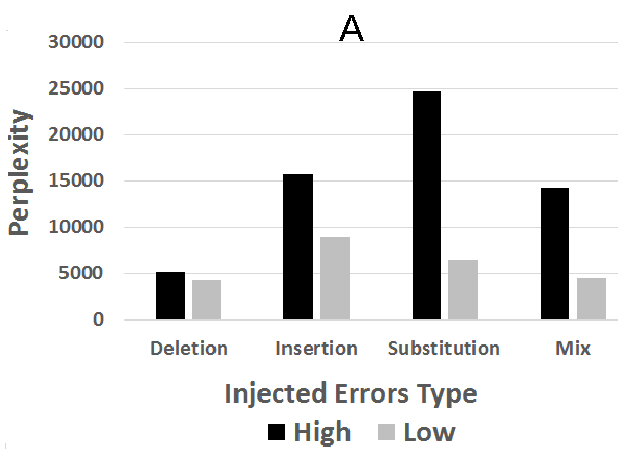
\includegraphics[width=\linewidth]{figs/Synth_NG_12.pdf}
 % \caption{A}
\end{minipage}%
\begin{minipage}[t]{.24\textwidth}
\centering
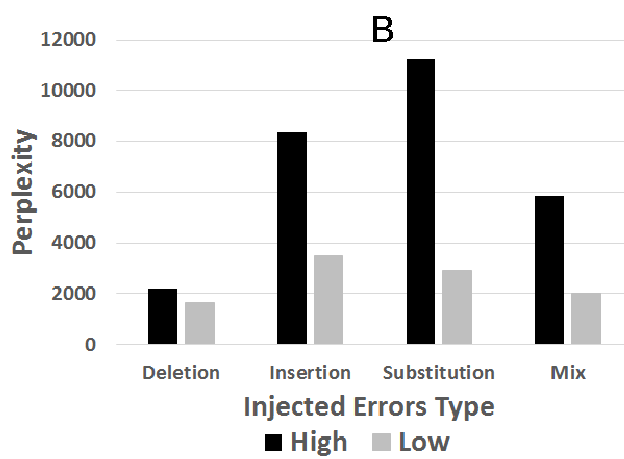
\includegraphics[width=\linewidth]{figs/Synth_NG_3.pdf}
 % \caption{B}
\end{minipage}%
\begin{minipage}[t]{.24\textwidth}
\centering
  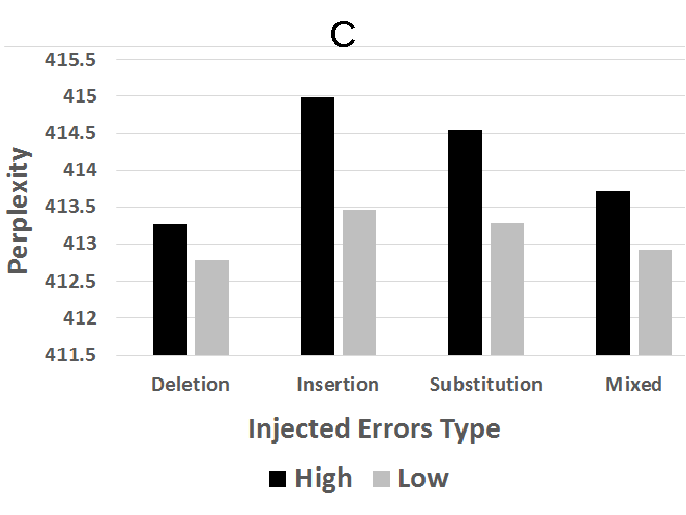
\includegraphics[width=\linewidth]{figs/Synth_RNN_12.pdf}
 % \caption{C}
\end{minipage}
\begin{minipage}[t]{.24\textwidth}
\centering
  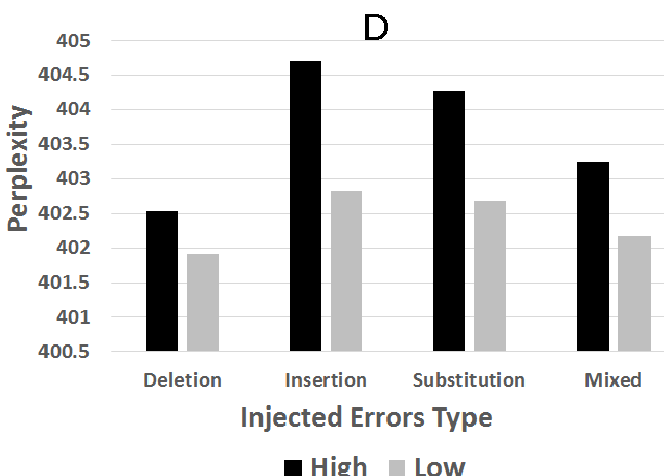
\includegraphics[width=\linewidth]{figs/Synth_RNN_3.pdf}
  %\caption{D}
\end{minipage}
\end{minipage}
  \caption{N-Gram (Figures A and B) and RNN (Figures C and D)  Perplexity metric for different types of synthetic errors: Indels and Substitution errors, and a mixture of the three for \textit{E. coli} str reference genome (Figures A and C) and \textit{Acinetobacter} sp. reference genome (Figures B and D). We compare two versions of such errors: high and low error rates.}
\label{figure:Synthetic_Errors_Detection}
\end{figure}

% \begin{figure}

% \end{figure}
% \begin{figure}
  
% \end{figure}


\end{document}

